\part{Advanced Topics in Controls and Physics}\label{part: advanced topics}
\begin{chapquote}{Claude Shannon}
    ``Mathematics is the tool specially suited for dealing with abstract concepts of any kind and there is no limit to its power in this field.''
\end{chapquote}

\newpage

\chapter*{Outline}

\color{red} This section is to be finished after the initial release of this volume. My apologies to any readers with particular interest in the methods of geometric control and differential geometry.\color{black}

In this final portion of the book, I will describe the methods of controls which are much beyond the standard coursework of a typical curriculum in engineering. This section will hold the information related to differential geometry, Lie theory, and it's application in the fields of geometric control (as well as some brief mention of the applications in physics). Such an understanding will require us to develop quite a bit of mathematics. The first several chapters will lay this mathematical foundation upon which our theories will be built.

This section is intended to live outside the scope of the rest of the book, such that the reader may stop their reading at the end of \autoref{part:control theory} and have gained all the necessary knowledge for a working understanding of control theory and energy mechanics. However, for those who want to dive deeply into these subject matter, this part will build off the rest of the book and dive into the study of advanced control theory and techniques. 

I start with a study of \gls{lie theory}, which will form a foundational knowledge of group theory and introduce us to the concepts of differentiable manifolds. From our study of \gls{lie theory}, the study of differentiable manifolds naturally arises. So, I devote this first section to a brief overview of Lie theory, differential geometry, and some applications. In fields such as geometric control, differential geometry plays a crucial part. The study of differential geometry should provide a satisfying unification of the ideas of Clifford algebras, \gls{lie theory}, and inner product spaces. It is truly one of the most profound mathematical generalizations of the ideas found in physics and engineering.

To supplement the information in this chapter, I have found that \cite{hirvonen_profound_nodate} has some quite readable and good articles on many of these topics. There are, of course, many other sources which are good for deep dives into any of these concepts.


\chapter{Lie Theory}\label{chap:lie theory}


\begin{chapquote}{Anthony Zee}
    ``It is almost as if the Creator of the universe understood Lie groups and decided to use them (a few of the simplest exemplars anyway) to construct the interactions among the fundamental particles that fill the universe. You
might call Him or Her an applied group theorist.''
\end{chapquote}
% \begin{chapquote}{Albert Camus}
%     ``If thought discovered in the shimmering mirrors of phenomena eternal relations capable of summing them up and summing themselves up in a single principle, then would be seen an intellectual joy of which the myth of the blessed would be but a ridiculous imitation.''
% \end{chapquote}

% clean up the notation for groups and ensure its all the same.

The goal until now has been to introduce the methods of \gls{Lagrangian} and \gls{Hamiltonian} mechanics and control theory in a way that does not require very rigorous mathematical formalisms. However, to tie up some of the loose ends, it is useful to introduce some mathematical concepts which can be used to understand these concepts on a more fundamental level. Along the way, we will also gain insight into the nature of rotations and curved spaces. Introducing these concepts will allow us to formalize huge swaths of the content covered in both Volume II and Volume III up to now, and will prove beneficial in the future endeavors of this volume as well.

This mathematical description is not strictly necessary to use the concepts mentioned throughout this book, but it is helpful for readers who hope to gain a full understanding of the content. I will warn that these chapters are likely the most technical in the book and will require significant effort from the reader. Throughout the chapter, I will slowly introduce the standard mathematical notation of proofs to use as a shorthand instead of writing everything out. This will help acquaint the reader if they are to read further on the subject matter discussed.

Since this is a heavy subject, supplemental resources will be useful. I have compiled a list of useful videos and texts to help explain \gls{lie theory}. Both of these video sources have good visuals that introduce \gls{lie theory} fairly intuitively. \cite{michael_penn_maths_2021} is more mathematically rigorous, but \cite{mathemaniac_what_2023} may be a better overall introduction. \gls{lie theory} is also used extensively in physics, so much material may be found in this domain. Two of my favorite sources in this domain are \cite{eigenchris_spinors_nodate} and \cite{zee_group_2016}.

For those readers who would like to dive deeper into the  subject or prefer written material to videos, I have included several good sources. Likely the best texts to read after this one is \cite{stillwell_naive_2008} and \cite{hall_lie_2015}, which both cover much of the basics of \gls{lie theory}.

\section{Motivation and Background}\label{sec:motivation and background lie}

Before we dive into the mathematical foundations of \gls{lie theory}, we should first examine why it is of importance to us. \gls{lie theory} is concerned with the inherit symmetries of mathematical objects. More specifically, the theory is concerned with so-called \textit{continuous symmetries}.

A big question is why do \textit{we} care? Well, it turns out that all of the rotations that we study are understood with \gls{lie theory}. It is also used to describe quaternions, symplectic groups (in Lagrangian and Hamiltonian mechanics), advanced control methods, robotics, and inertial navigation, just to name a few use cases. Gaining an intuition for the underlying mathematics will prove useful for us. 

For us, \gls{lie theory} is especially useful in our study of dynamic systems. Often, we do have symmetries in our problems. There are those symmetries that are obvious -- such as axial symmetry and reflectional symmetry of an object. There are deeper, more fundamental symmetries though, such as the symmetry between the rotational invariance of the Lagrangian and conservation of angular momentum (we will explore this more in \autoref{Noether's Theorem}).

Understanding symmetries is what led Sophus Lie to originally develop his theory. The study of discrete symmetries by Galois had proven very useful in understanding polynomial equations. Originally, Sophus Lie (shown in \autoref{fig:Lie}) developed the theory in order to understand the continuous symmetries of differential equations. However, the theory also proved to be useful in describing other symmetries, such as the rotations and conservation equations which we are familiar with in dynamics.

\begin{figure}[ht]
    \centering
    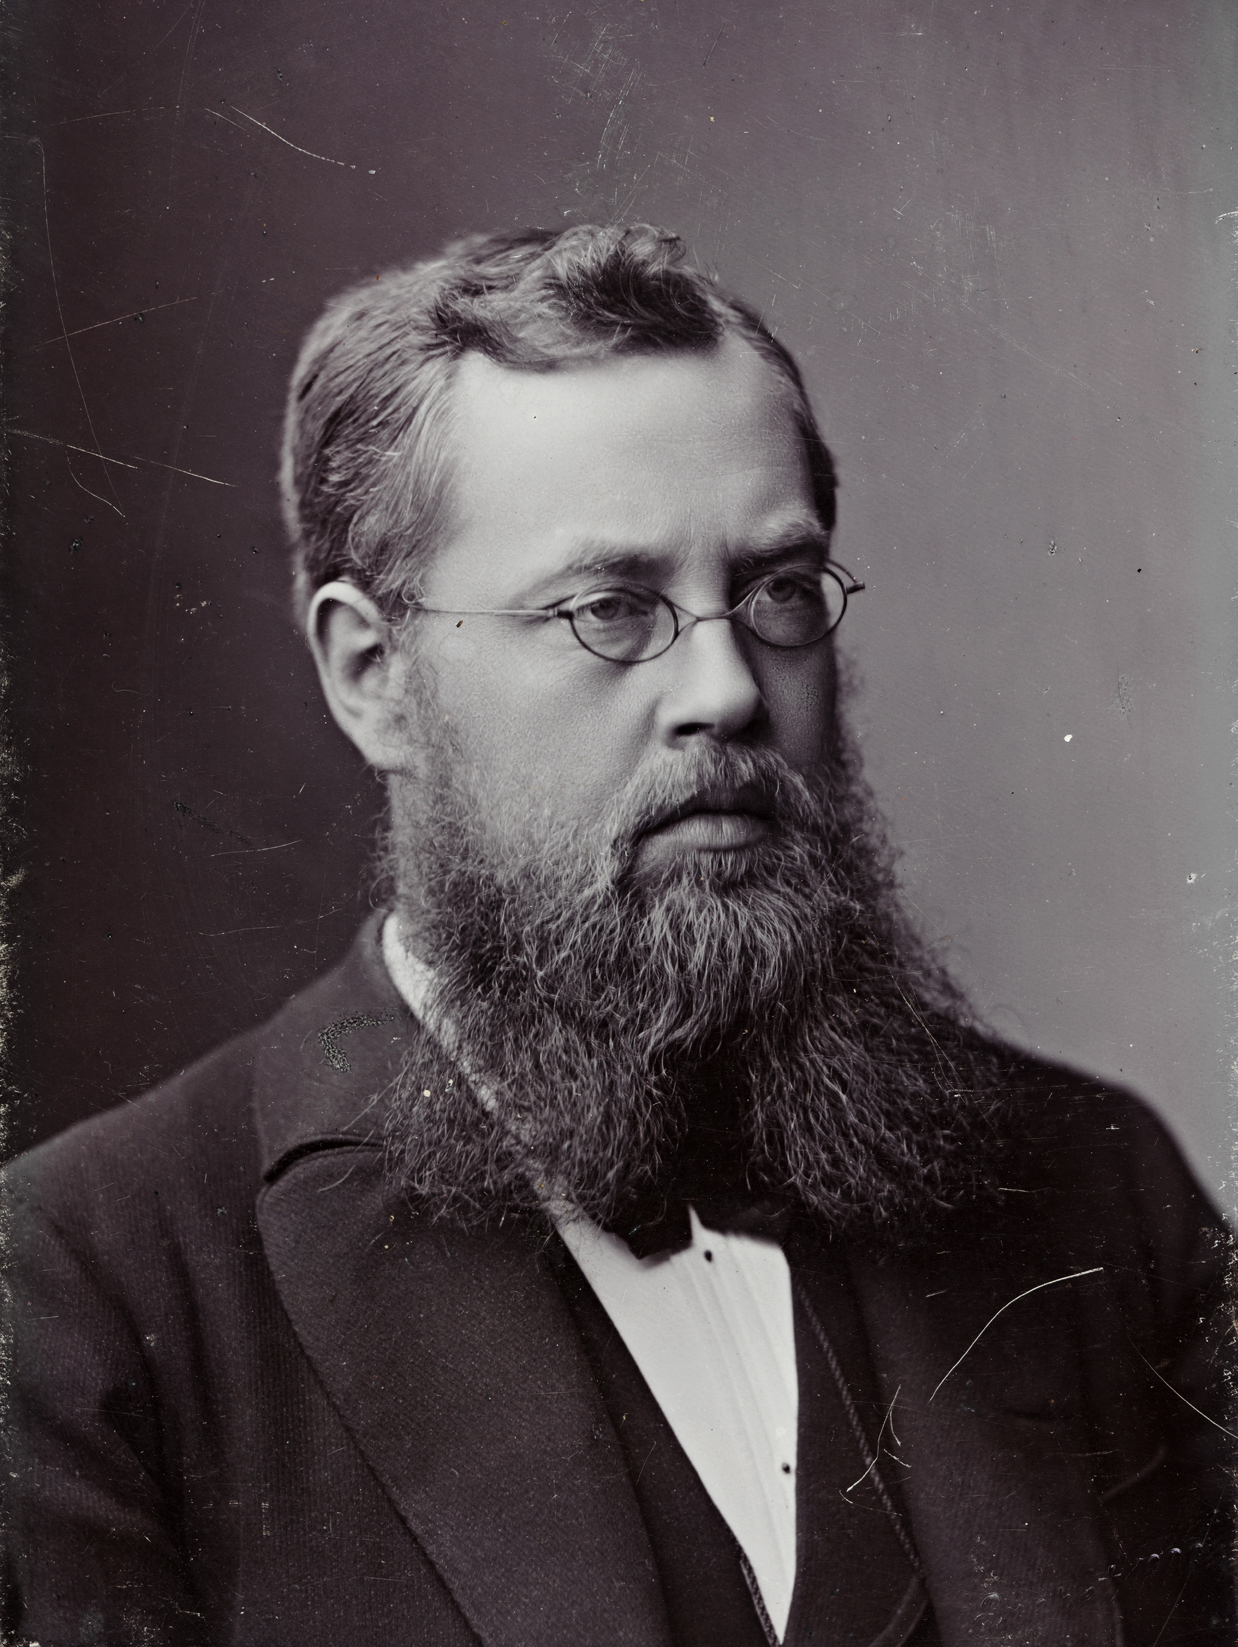
\includegraphics[width=0.5\linewidth]{Images/Portrett_av_Sophus_Lie.jpg}
    \caption{A Portrait of Sophus Lie}
    \label{fig:Lie}
\end{figure}

The big question, then, is how we can describe symmetry mathematically. A mathematical object known as a \textit{group} is the answer. Groups contain inherit information about symmetry. Lie theory extends this concept via the inclusion of \textit{manifolds} - which will be detailed later. The important conceptual understanding is that groups provide the symmetry, and the manifolds give a `language' to describe our system using a set of coordinates - much like we can describe any point on the surface of earth using latitude and longitude.\endnote{Some mathematicians will be quick to point out that manifolds don't necessarily need coordinates for their description. For calculations, however, we like to ascribe these qualities. In physics, it is typical that we use cartesian coordinates when we do this conversion to physical units, since they require no Jacobian.}

The other big part of \gls{lie theory} is that we can describe the attributes of our system at a point using \textit{algebras}. By thinking about our system as a manifold, we are able to describe coordinates for a certain location. Then, we can do something akin to a derivative - looking at the space `tangent' to the manifold at that point. This `tangent space' is what we call the \gls{lie algebra}.

\glspl{lie algebra} are useful because the tangent space is flat. Because it is flat, typical rules of geometry and calculus can be used, making analysis much easier. These algebras are essentially our computational tool that allows us to do simple calculations that yield complex results.

The last important thing to mention is that we can convert between the \gls{lie group} and the \gls{lie algebra} using something called an \gls{exponential map}. For some groups and operations, this \gls{exponential map} is simply an exponential function. Other times, however, we need a different way to describe these exponential transformations. This will be discussed later.

The most important thing to realize is that we can relate a complex non-linear system (represented in \gls{lie theory} by a group on a manifold) locally with a linearized version of the system, which we essentially `project' onto the system via the \gls{exponential map}. 

We've just gone through the premise of \gls{lie theory} at a blistering speed. We will dive into each aspect in much greater detail in the following chapters. What is important now is to understand the big picture ideas as we construct our mathematical ideas.

As a final point before we start, I believe that Lie theory is simply a beautiful theory which ties together so much mathematics. A careful study of Lie theory will unite many of the mathematical concepts you encounter.

\section{Groups and Symmetries}
\begin{chapquote}{Mark A. Armstrong}
    ``Numbers measure size, groups measure symmetry''
\end{chapquote}

Groups are extremely fundamental in the construction of Lie theory. As we have mentioned, groups provide the language of symmetries. They are conceptually simple but exceedingly powerful.\endnote{In fact, we see groups used very often in quantum mechanics and field theories. Groups are foundational in our understanding of why forces themselves exist!}

Before we get to formal definitions, it is helpful to have a mental picture of what a group is. From there, we can narrow our view to the concept of a  \gls{lie group}. 2-D Shapes are a good motivating example for what groups are at the basic level. We can consider a basic shape, like the equilateral triangle, as an example. What we define as the \textit{group} is the collection of symmetries that the triangle exhibits.

\begin{example}[The Symmetries of a Triangle]
A triangle is a good showcase of the symmetries that we find naturally in geometry. Let us consider an equilateral triangle as shown in \autoref{fig:eq triangle}.

\begin{figure}[H]
    \centering

\tikzset{every picture/.style={line width=0.75pt}} %set default line width to 0.75pt        

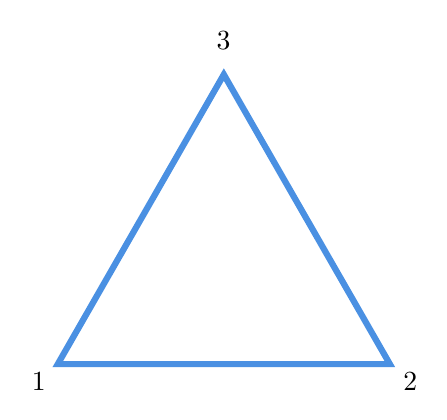
\begin{tikzpicture}[x=0.75pt,y=0.75pt,yscale=-1,xscale=1]
%uncomment if require: \path (0,300); %set diagram left start at 0, and has height of 300

%Shape: Triangle [id:dp8868857688850825] 
\draw  [color={rgb, 255:red, 74; green, 144; blue, 226 }  ,draw opacity=1 ][line width=2.25]  (330,70.47) -- (410,210) -- (250,210) -- cycle ;

% Text Node
\draw (236,212.4) node [anchor=north west][inner sep=0.75pt]    {$1$};
% Text Node
\draw (415,212.4) node [anchor=north west][inner sep=0.75pt]    {$2$};
% Text Node
\draw (325,48.4) node [anchor=north west][inner sep=0.75pt]    {$3$};

\end{tikzpicture}

    \caption{An Equilateral Triangle}
    \label{fig:eq triangle}
\end{figure}

It is natural to say that this triangle is symmetric, but what do we really mean when we say that? Mathematically, we're saying that we can perform some operation, which we may call $g$, and the result is that the triangle looks exactly identical afterward. 

The vertices of this triangle have only been labeled so that we can keep track of them as we perform actions on this triangle. If we don't have these labels, we couldn't see anything changing. This highlights one important thing about groups -- our group operations are those operations where we look at our object and we observe no measurable change.

Let's understand each symmetry of the triangle one at a time. We'll start with reflectional symmetries, like putting the triangle in a mirror. We can reflect about the vertical line through `3' as an example of such a symmetry.
\begin{figure}[H]
    \centering
    

\tikzset{every picture/.style={line width=0.75pt}} %set default line width to 0.75pt        

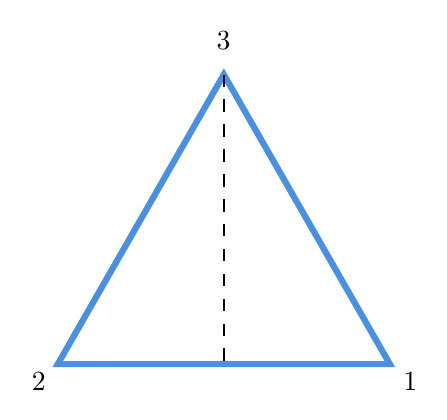
\begin{tikzpicture}[x=0.75pt,y=0.75pt,yscale=-1,xscale=1]
%uncomment if require: \path (0,300); %set diagram left start at 0, and has height of 300

%Shape: Triangle [id:dp8868857688850825] 
\draw  [color={rgb, 255:red, 74; green, 144; blue, 226 }  ,draw opacity=1 ][line width=2.25]  (330,70.47) -- (410,210) -- (250,210) -- cycle ;
%Straight Lines [id:da17313732782624203] 
\draw  [dash pattern={on 4.5pt off 4.5pt}]  (330,70.47) -- (330,210) ;

% Text Node
\draw (236,212.4) node [anchor=north west][inner sep=0.75pt]    {$2$};
% Text Node
\draw (415,212.4) node [anchor=north west][inner sep=0.75pt]    {$1$};
% Text Node
\draw (325,48.4) node [anchor=north west][inner sep=0.75pt]    {$3$};


\end{tikzpicture}
    \caption{Reflectional Symmetry of Triangle}
    \label{fig:triangle reflect}
\end{figure}
We can see that this action flips the locations of `1' and `2', but if we had not designated these points, we'd have no way of knowing the triangle was changed! For this reason, we call this action a symmetry of the triangle.

We can also rotate the triangle by $120
\degree$ about it's geometric center to get another indistinguishable triangle.
\begin{figure}[H]
    \centering

\tikzset{every picture/.style={line width=0.75pt}} %set default line width to 0.75pt        

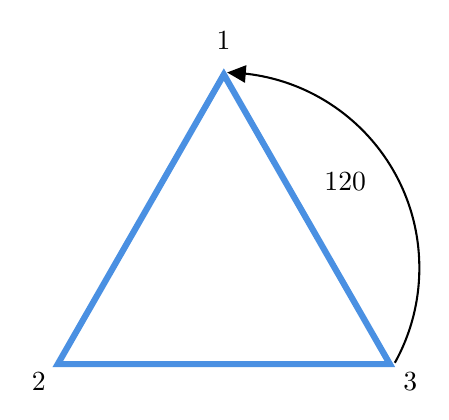
\begin{tikzpicture}[x=0.75pt,y=0.75pt,yscale=-1,xscale=1]
%uncomment if require: \path (0,300); %set diagram left start at 0, and has height of 300

%Shape: Triangle [id:dp021503950787327253] 
\draw  [color={rgb, 255:red, 74; green, 144; blue, 226 }  ,draw opacity=1 ][line width=2.25]  (330,70.47) -- (410,210) -- (250,210) -- cycle ;
%Shape: Arc [id:dp6942684746026092] 
\draw  [draw opacity=0] (331.64,69.49) .. controls (382.91,70.36) and (424.2,112.19) .. (424.2,163.67) .. controls (424.2,180.24) and (419.92,195.82) .. (412.4,209.35) -- (330,163.67) -- cycle ; \draw    (334.71,69.59) .. controls (384.54,72.04) and (424.2,113.22) .. (424.2,163.67) .. controls (424.2,180.24) and (419.92,195.82) .. (412.4,209.35) ;  \draw [shift={(331.64,69.49)}, rotate = 4.65] [fill={rgb, 255:red, 0; green, 0; blue, 0 }  ][line width=0.08]  [draw opacity=0] (8.93,-4.29) -- (0,0) -- (8.93,4.29) -- cycle    ;

% Text Node
\draw (236,212.4) node [anchor=north west][inner sep=0.75pt]    {$2$};
% Text Node
\draw (415,212.4) node [anchor=north west][inner sep=0.75pt]    {$3$};
% Text Node
\draw (325,48.4) node [anchor=north west][inner sep=0.75pt]    {$1$};
% Text Node
\draw (377,116.4) node [anchor=north west][inner sep=0.75pt]    {$120\degree $};


\end{tikzpicture}

    \caption{Rotational Symmetry of a Triangle}
    \label{fig:rot triangle}
\end{figure}
In total, there are 6 ways that we can create a triangle which looks exactly the same as the one we started with. All of these are shown in \autoref{fig:sym tri}.
\begin{figure}[H]
    \centering
    

\tikzset{every picture/.style={line width=0.75pt}} %set default line width to 0.75pt        

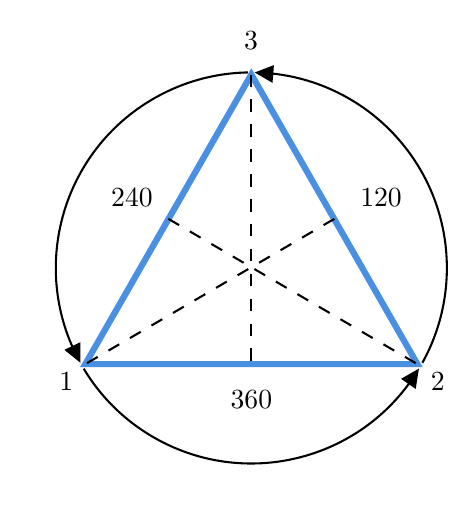
\begin{tikzpicture}[x=0.75pt,y=0.75pt,yscale=-1,xscale=1]
%uncomment if require: \path (0,300); %set diagram left start at 0, and has height of 300

%Shape: Triangle [id:dp021503950787327253] 
\draw  [color={rgb, 255:red, 74; green, 144; blue, 226 }  ,draw opacity=1 ][line width=2.25]  (330,70.47) -- (410,210) -- (250,210) -- cycle ;
%Shape: Arc [id:dp6942684746026092] 
\draw  [draw opacity=0] (331.64,69.49) .. controls (382.91,70.36) and (424.2,112.19) .. (424.2,163.67) .. controls (424.2,180.24) and (419.92,195.82) .. (412.4,209.35) -- (330,163.67) -- cycle ; \draw    (334.71,69.59) .. controls (384.54,72.04) and (424.2,113.22) .. (424.2,163.67) .. controls (424.2,180.24) and (419.92,195.82) .. (412.4,209.35) ;  \draw [shift={(331.64,69.49)}, rotate = 4.65] [fill={rgb, 255:red, 0; green, 0; blue, 0 }  ][line width=0.08]  [draw opacity=0] (8.93,-4.29) -- (0,0) -- (8.93,4.29) -- cycle    ;
%Shape: Arc [id:dp18064647912182097] 
\draw  [draw opacity=0] (410.74,212.18) .. controls (384.35,256.14) and (327.48,270.98) .. (282.9,245.25) .. controls (268.55,236.96) and (257.2,225.47) .. (249.24,212.19) -- (330,163.67) -- cycle ; \draw    (409.12,214.79) .. controls (382.08,256.72) and (326.59,270.47) .. (282.9,245.25) .. controls (268.55,236.96) and (257.2,225.47) .. (249.24,212.19) ;  \draw [shift={(410.74,212.18)}, rotate = 124.65] [fill={rgb, 255:red, 0; green, 0; blue, 0 }  ][line width=0.08]  [draw opacity=0] (8.93,-4.29) -- (0,0) -- (8.93,4.29) -- cycle    ;
%Shape: Arc [id:dp048284149806032906] 
\draw  [draw opacity=0] (247.61,209.34) .. controls (222.74,164.5) and (238.32,107.83) .. (282.9,82.09) .. controls (297.25,73.81) and (312.88,69.73) .. (328.36,69.47) -- (330,163.67) -- cycle ; \draw    (246.17,206.63) .. controls (223.37,162.25) and (239.21,107.31) .. (282.9,82.09) .. controls (297.25,73.81) and (312.88,69.73) .. (328.36,69.47) ;  \draw [shift={(247.61,209.34)}, rotate = 244.65] [fill={rgb, 255:red, 0; green, 0; blue, 0 }  ][line width=0.08]  [draw opacity=0] (8.93,-4.29) -- (0,0) -- (8.93,4.29) -- cycle    ;
%Straight Lines [id:da4638366372358793] 
\draw  [dash pattern={on 4.5pt off 4.5pt}]  (330,70.47) -- (330,210) ;
%Straight Lines [id:da9032255747155441] 
\draw  [dash pattern={on 4.5pt off 4.5pt}]  (290,140) -- (410,210) ;
%Straight Lines [id:da6037792210940448] 
\draw  [dash pattern={on 4.5pt off 4.5pt}]  (370,140) -- (250,210) ;

% Text Node
\draw (236,212.4) node [anchor=north west][inner sep=0.75pt]    {$1$};
% Text Node
\draw (415,212.4) node [anchor=north west][inner sep=0.75pt]    {$2$};
% Text Node
\draw (325,48.4) node [anchor=north west][inner sep=0.75pt]    {$3$};
% Text Node
\draw (284,130) node [anchor=east] [inner sep=0.75pt]    {$240\degree $};
% Text Node
\draw (330,221.4) node [anchor=north] [inner sep=0.75pt]    {$360\degree $};
% Text Node
\draw (381,130) node [anchor=west] [inner sep=0.75pt]    {$120\degree $};

\end{tikzpicture}

    \caption{Symmetries of the Trangle}
    \label{fig:sym tri}
\end{figure}
    The very special thing about these symmetries is that we can do two (or more) of them -- one after the other -- and we get another symmetry of the group. Go ahead and try it! You'll find that no matter which operations you do, there's always a way to accomplish it with a single operation! This very special property is called \textit{closure}.
    There is one other thing, too

    One last thing to note: you'll notice that a rotation by $360\degree$ is equivalent to rotation by $0\degree$. This rotation effectively `does nothing'. This is what we call the identity element. Although it seems simple, it is a very important part of the group.

    This brief introduction should give you everything you need to help motivate the axiomatic treatment of groups and the \glspl{lie group} that are to follow.

    If you want more practice or explanation with these concepts, 3Blue1Brown has a good video to help introduce this concept, which has be found at \cite{3blue1brown_eulers_2017}.
\end{example}

What we have just seen with the triangle is an example of a \textit{discrete symmetry}; a symmetry which requires us to do a sort of `jump' to reach our next symmetry. Since the symmetry is discrete, we can count the total number of symmetries that we have. In the case of the triangle, we have our three rotations and three reflections, giving us a countable set of symmetries.

There is another type of symmetry that exists, and one that will in fact be far more useful for us. This type of symmetry is a \textit{continuous symmetry}. Sticking with our 2-D shapes, we can think about a circle instead:
\begin{figure}[ht]
    \centering

\tikzset{every picture/.style={line width=0.75pt}} %set default line width to 0.75pt        

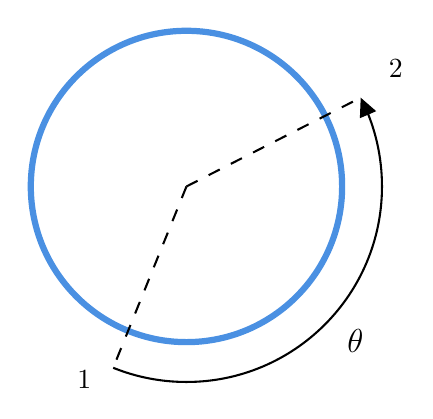
\begin{tikzpicture}[x=0.75pt,y=0.75pt,yscale=-1,xscale=1]
%uncomment if require: \path (0,300); %set diagram left start at 0, and has height of 300

%Shape: Circle [id:dp012698292168043301] 
\draw  [color={rgb, 255:red, 74; green, 144; blue, 226 }  ,draw opacity=1 ][line width=2.25]  (250,135) .. controls (250,93.58) and (283.58,60) .. (325,60) .. controls (366.42,60) and (400,93.58) .. (400,135) .. controls (400,176.42) and (366.42,210) .. (325,210) .. controls (283.58,210) and (250,176.42) .. (250,135) -- cycle ;
%Shape: Arc [id:dp4686733674855805] 
\draw  [draw opacity=0] (408.95,92.23) .. controls (415.5,105.06) and (419.2,119.6) .. (419.2,135) .. controls (419.2,187.02) and (377.02,229.2) .. (325,229.2) .. controls (312.52,229.2) and (300.6,226.77) .. (289.7,222.36) -- (325,135) -- cycle ; \draw    (410.28,94.95) .. controls (416,107.1) and (419.2,120.68) .. (419.2,135) .. controls (419.2,187.02) and (377.02,229.2) .. (325,229.2) .. controls (312.52,229.2) and (300.6,226.77) .. (289.7,222.36) ;  \draw [shift={(408.95,92.23)}, rotate = 66.66] [fill={rgb, 255:red, 0; green, 0; blue, 0 }  ][line width=0.08]  [draw opacity=0] (8.93,-4.29) -- (0,0) -- (8.93,4.29) -- cycle    ;
%Straight Lines [id:da10366016362761077] 
\draw  [dash pattern={on 4.5pt off 4.5pt}]  (325,135) -- (289.7,222.36) ;
%Straight Lines [id:da8482728300676312] 
\draw  [dash pattern={on 4.5pt off 4.5pt}]  (325,135) -- (408.95,92.23) ;

% Text Node
\draw (271,222.4) node [anchor=north west][inner sep=0.75pt]    {$1$};
% Text Node
\draw (421,72.4) node [anchor=north west][inner sep=0.75pt]    {$2$};
% Text Node
\draw (401,202.4) node [anchor=north west][inner sep=0.75pt]  [font=\large]  {$\theta $};


\end{tikzpicture}


    \caption{Symmetries of a circle}
    \label{fig:circle sym}
\end{figure}

In contrast with the triangle, this circle may be rotated through \textit{any} angle or reflected about any axis. Mathematically, what makes this different is that it requires no `jump' to go from one symmetry to the next. Our symmetries are continuous as we go around the circle. In fact, the circle group, which we often denote $\mathbb{S}^1$, is one of the prototypical examples of a \gls{lie group}. This smoothly varying structure is in fact the definitive concept us to define this as a \gls{lie group}.
\footnote{If you want to dive deeper into group theory, a wonderful introductory text can be found in \cite{armstrong_groups_1988}.}

\section{Lie Groups}
The \gls{lie group} is in essence a group and a manifold, which is shown in \autoref{fig:Lie Group}:
\begin{figure}[ht]
    \centering





% Gradient Info
  
\tikzset {_5g6glwol0/.code = {\pgfsetadditionalshadetransform{ \pgftransformshift{\pgfpoint{93.6 bp } { -132.6 bp }  }  \pgftransformscale{1.04 }  }}}
\pgfdeclareradialshading{_kg48z90ds}{\pgfpoint{-96bp}{136bp}}{rgb(0bp)=(1,1,1);
rgb(0bp)=(1,1,1);
rgb(25bp)=(0.29,0.56,0.89);
rgb(400bp)=(0.29,0.56,0.89)}
\tikzset{_v4ek6umsw/.code = {\pgfsetadditionalshadetransform{\pgftransformshift{\pgfpoint{93.6 bp } { -132.6 bp }  }  \pgftransformscale{1.04 } }}}
\pgfdeclareradialshading{_66pto071l} { \pgfpoint{-96bp} {136bp}} {color(0bp)=(transparent!40);
color(0bp)=(transparent!40);
color(25bp)=(transparent!50);
color(400bp)=(transparent!50)} 
\pgfdeclarefading{_h77ttbdia}{\tikz \fill[shading=_66pto071l,_v4ek6umsw] (0,0) rectangle (50bp,50bp); } 
\tikzset{every picture/.style={line width=0.75pt}} %set default line width to 0.75pt        

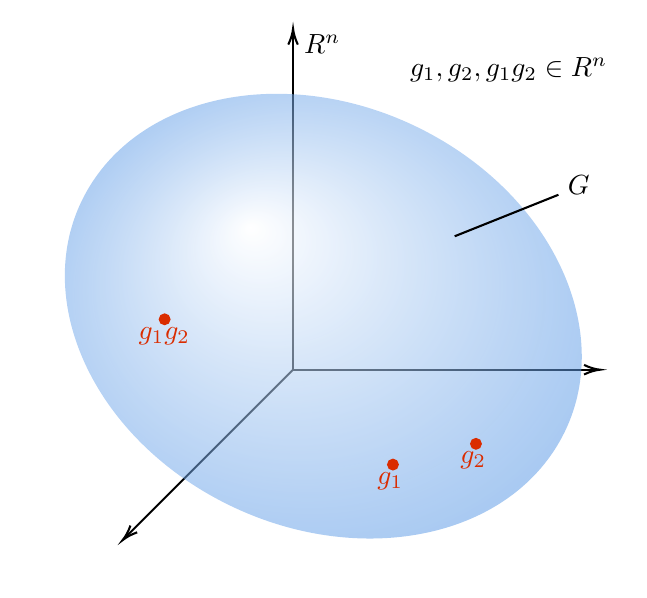
\begin{tikzpicture}[x=0.75pt,y=0.75pt,yscale=-1,xscale=1]
%uncomment if require: \path (0,300); %set diagram left start at 0, and has height of 300

%Straight Lines [id:da6341386319589457] 
\draw    (292.14,174.29) -- (292.14,12) ;
\draw [shift={(292.14,10)}, rotate = 90] [color={rgb, 255:red, 0; green, 0; blue, 0 }  ][line width=0.75]    (7.65,-2.3) .. controls (4.86,-0.97) and (2.31,-0.21) .. (0,0) .. controls (2.31,0.21) and (4.86,0.98) .. (7.65,2.3)   ;
%Straight Lines [id:da24449585878217006] 
\draw    (292.14,174.29) -- (438,174.29) ;
\draw [shift={(440,174.29)}, rotate = 180] [color={rgb, 255:red, 0; green, 0; blue, 0 }  ][line width=0.75]    (7.65,-2.3) .. controls (4.86,-0.97) and (2.31,-0.21) .. (0,0) .. controls (2.31,0.21) and (4.86,0.98) .. (7.65,2.3)   ;
%Straight Lines [id:da20393695102666232] 
\draw    (292.14,174.29) -- (211.41,255.01) ;
\draw [shift={(210,256.43)}, rotate = 315] [color={rgb, 255:red, 0; green, 0; blue, 0 }  ][line width=0.75]    (7.65,-2.3) .. controls (4.86,-0.97) and (2.31,-0.21) .. (0,0) .. controls (2.31,0.21) and (4.86,0.98) .. (7.65,2.3)   ;

%Shape: Donut [id:dp3968285728219174] 
\draw  [draw opacity=0][shading=_kg48z90ds,_5g6glwol0,path fading= _h77ttbdia ,fading transform={xshift=2}] (283.14,135.41) .. controls (283.14,135.41) and (293.7,141.26) .. (306.72,148.48) .. controls (319.74,155.7) and (330.3,161.55) .. (330.3,161.55) .. controls (330.3,161.55) and (319.74,155.7) .. (306.72,148.48) .. controls (293.7,141.26) and (283.14,135.41) .. (283.14,135.41)(194.07,86.04) .. controls (223.35,37.96) and (297.53,26.94) .. (359.75,61.43) .. controls (421.97,95.92) and (448.66,162.85) .. (419.37,210.93) .. controls (390.09,259) and (315.91,270.02) .. (253.69,235.53) .. controls (191.47,201.04) and (164.78,134.11) .. (194.07,86.04) ;
%Straight Lines [id:da060154956904347356] 
\draw [color={rgb, 255:red, 218; green, 44; blue, 0 }  ,draw opacity=1 ]   (340.26,220) ;
\draw [shift={(340.26,220)}, rotate = 0] [color={rgb, 255:red, 218; green, 44; blue, 0 }  ,draw opacity=1 ][fill={rgb, 255:red, 218; green, 44; blue, 0 }  ,fill opacity=1 ][line width=0.75]      (0, 0) circle [x radius= 2.34, y radius= 2.34]   ;
%Straight Lines [id:da47247361109034747] 
\draw [color={rgb, 255:red, 218; green, 44; blue, 0 }  ,draw opacity=1 ]   (380.26,210) ;
\draw [shift={(380.26,210)}, rotate = 0] [color={rgb, 255:red, 218; green, 44; blue, 0 }  ,draw opacity=1 ][fill={rgb, 255:red, 218; green, 44; blue, 0 }  ,fill opacity=1 ][line width=0.75]      (0, 0) circle [x radius= 2.34, y radius= 2.34]   ;
%Straight Lines [id:da7815998594768269] 
\draw [color={rgb, 255:red, 218; green, 44; blue, 0 }  ,draw opacity=1 ]   (230.26,150) ;
\draw [shift={(230.26,150)}, rotate = 0] [color={rgb, 255:red, 218; green, 44; blue, 0 }  ,draw opacity=1 ][fill={rgb, 255:red, 218; green, 44; blue, 0 }  ,fill opacity=1 ][line width=0.75]      (0, 0) circle [x radius= 2.34, y radius= 2.34]   ;
%Straight Lines [id:da8835218032244371] 
\draw    (370,110) -- (420,90) ;

% Text Node
\draw (331.26,222.4) node [anchor=north west][inner sep=0.75pt]  [color={rgb, 255:red, 218; green, 44; blue, 0 }  ,opacity=1 ]  {$g_{1}$};
% Text Node
\draw (371.26,212.4) node [anchor=north west][inner sep=0.75pt]  [color={rgb, 255:red, 218; green, 44; blue, 0 }  ,opacity=1 ]  {$g_{2}$};
% Text Node
\draw (216.26,152.4) node [anchor=north west][inner sep=0.75pt]  [color={rgb, 255:red, 218; green, 44; blue, 0 }  ,opacity=1 ]  {$g_{1} g_{2}$};
% Text Node
\draw (296,11.4) node [anchor=north west][inner sep=0.75pt]    {$\mathbb{R}^{n}$};
% Text Node
\draw (347,22.4) node [anchor=north west][inner sep=0.75pt]    {$g_{1} ,g_{2} ,g_{1} g_{2} \in \mathbb{R}^{n}$};
% Text Node
\draw (423,79.4) node [anchor=north west][inner sep=0.75pt]    {$G$};


\end{tikzpicture}



    \caption{Visualization of the Lie Group}
    \label{fig:Lie Group}
\end{figure}
What exactly does it mean for the \gls{lie group} to be both a group and a manifold?

The blue `orb' denoted $G$ is representative of a smooth manifold in $\mathbb{R}^n$. We can think of the manifold in this example as the surface of a 2D ellipsoid on which all the members of the group must live. We can see three points defined $g_1$, $g_2$, and $g_1\cdot g_2$. In this example, $g_1\cdot g_2$ is simply the multiplication of $g_1$ and $g_2$. We can remember from our triangle example that the product $g_1\cdot g_2$ must also be in the group because of closure.

The property that must hold for a \gls{lie group} is that not only do all $g_1,g_2,g_1\cdot g_2$ reside in $\mathbb{R}^n$, but additionally also lie on the surface of the ellipsoid! In other words, $g_1,g_2,g_1\cdot g_2\in G$. Now that we have a mental picture, we can move on to the formal definition.

\subsection{The Axioms of Groups}
As mentioned before, the defining feature of the \gls{lie group} is that it is both a group and a manifold. We must first define the attributes of a group if we are to formally define this concept. 

A group is a mathematical \textit{set} which obeys the following four properties for a given \textit{binary operation}. These properties are shown formally and then explained afterward.

\begin{enumerate}
\item $Closure{:} \mathrm{\ for \ all\ } g,h \in G, g\cdot h \in G$
\item $Associativity{:} \mathrm{\ for \ all \ } g,h,k \in  G, (g\cdot h)\cdot k=g\cdot(h\cdot k)$
\item $Identity{:} \mathrm{\ there \ is  \ } e\in G, \mathrm{\ for \ all \ } g \in G, e\cdot g=g\cdot e=g$
\item $Inverse{:} \mathrm{\ for \ all \ } g \in G, \mathrm{\ there \ is  \ } h \in G, g \cdot h=h\cdot g =e$
\end{enumerate}


I will now go over all of these properties to explain their meaning in more natural language for readers not familiar with the notation above.

\begin{enumerate}
    \item By closure, we mean that when we apply an operation on a \textit{set}, we get another element of that set. This is best motivated by an example. 

    Let us take the natural numbers, denoted $\mathbb{N}$ to be our set. The natural numbers are given as $1,2,3\cdots$  and so on. We say that the natural numbers are closed under addition, because adding any of the elements of the set together, we get another element of the set. For example, adding $1$ and $3$, we get $4$, which is also in the set $\mathbb{N}$. Moreover, any composition of these operations will also be part of the set. Performing addition twice will still give an element of the sequence. 
    
    Connecting this to our notation, we say that two elements, $g$ and $h$ are in the set $G$, which we represent with this notation: $g,h \in G$. We define the operation to be `$\cdot$', which is the notation for a general operation. We can then say that the elements, when acted upon by this operation, are still in the set $G$: $g\cdot h \in G$. This is what the formal definition of closure is.
    \item Associativity is a more simple concept which most readers are likely familiar with. It simply means that the grouping of the operations does not matter. Note that associativity \textit{does not} imply communitivity! If we take the example of matrices, $(AB)C=A(BC)$, which is an expression of associativity, but $AB\neq BA$ for matrices. 
    \item Identity is also relatively simple. Identity simply means that there exists an element of the set $G$, which when applied on another element of set $G$, has no effect. For the real numbers, $\mathbb{R}$, multiplication by the number $1$ is an example of an identity element.
    \item Inverse is the last property, which states that for each element in the set, there is another element in the set, that when acted upon by an operation, returns the identity. This is analogous to the inverse of a number, or inverse of a function, which you have studied in algebra.
\end{enumerate}

Lastly, I will explain what a \textit{binary operation} is. Stated simply, a binary operation is an operation which takes in two inputs and returns a single output. Most operations, such as addition, subtraction, and multiplication are binary. Basically, a binary operation is a simple mathematical operation between two numbers that you are familiar with.

\subsubsection{Further Group Examples}

Let's solidify our understanding of groups with some examples. Some of these are worked examples (blue), and some will require the reader to work through them (red).

\begin{example}[The Real Numbers]
    To wrap our minds around the concepts of groups, we consider the example of the integers, $\mathbb{Z}$.

    To check if the integers form a group, we first need to define our operation. We will choose addition. Then, we simply check each of the properties. 
    
    We have shown previously that adding any two natural numbers gives another natural number, and we can intuitively extend this to the integers as well. Next, we consider the associativity. It is easily seen that $(a+b)+c=a+(b+c)$, since addition is associative. Next, we consider the identity. For the operation of addition, the identity is the number $0$, which when added to any integer, $z$, does nothing. Lastly, we consider the inverse. We should have for every integer another integer such that $a+b=0$. It is obvious that $b=-a$, which is satisfied since the integers include negative numbers. Thus, we have shown that the integers are closed under addition.
\end{example}

The axioms of groups can be applied to create a group from any set of objects. In our study, it is most helpful to assign group identities to matrices, since our studies of rotations and control systems involve matrices heavily.

\begin{exercise}
We have shown in the previous example how the real numbers are closed under addition. Using the same axiomatic approach,  show why the integers are not a group under multiplication. Which axiom(s) is/are violated?
\end{exercise}

\begin{exercise}
    We have shown that we can make groups out of the elements of the number line. Previously, we have stated that groups contain information about symmetries. Think about the symmetries that are associated with the number line. How are these different than the symmetries associated with geometry? 
    
    Symmetries, typically, are quite broad! Here are just a few examples that you can try. See if you can explain what symmetries may exist for these objects:
    \begin{itemize}
        \item Functions (even, odd)
        \item Matrices
        \item Taylor Series
    \end{itemize}
There are many more types of symmetries which you may encounter if you further study mathematics!
\end{exercise}



\begin{example}[The Quaternion Group]
We have shown in Volume II that the quaternions form an algebra which we call $\mathbb{H}$. We define the elements of $\mathbb{H}$:
$q=q_0+q_1i+q_2j+q_3k ,\quad q_0,q_1,q_2,q_3\in\mathbb{R}$
    More specifically, this algebra is a four-dimensional associate unital algebra. We have the four dimensions defined by the basis: $1,i,j,k$. These elements are associative, meaning that the order in which we perform operations does not matter (However, the operations are not commutative!). Unital simply means that the algebra contains an identity element.

    We can again show all of the properties of the \gls{lie group} hold for the quaternion algebra.

    \begin{enumerate}
        \item Closure: We can show the closure of the group by considering the multiplication of any element of the quaternion group with any other element.
$$\begin{array}{c|cccc}
     \times&1&i&j&k  \\
     \hline
     1&1&i&j&k\\
     i&i&-1&k&-j\\
     j&j&-k&-1&i\\
     k&k&j&-i&-1\\
\end{array}$$
As we can see, the there is no multiplication that we can do that gives an element outside of the group. Therefore, the quaternions are closed under multiplication.
\item Associativity: An exact proof of the associativity of quaternions follows from the Cayley-Dickson construction of the quaternions or from Clifford algebras (which are discussed in Volume II). This is not immediately evident, but it is true that the quaternions are associative. More information can be found in \cite{michael_penn_climbing_2023} for the approach using the Cayley-Dickson construction or in \cite{sudgylacmoe_swift_2020} for the approach using Clifford algebras.
\item Identity: The identity element of the quaternions is simple, it is the element which contains only a real part of 1 and no other element.
\item Inverse: The inverse for the quaternions is also fairly simple. We can see from the multiplication table that any element of the quaternion algebra multiplied by itself gives the negative of the identity. So, we can simply multiply one of these terms by $-1$ to construct the identity. Since $-1$ is in the span of the real numbers, this is perfectly fine to do!


    \end{enumerate}
    So we have shown that the quaternions form both an algebra and a group! This is a quite interesting property. See if there are any other common mathematical objects that you can find group representations for!
\end{example}

\begin{exercise}[The Octonion Group (Hard)]

The octonions are an example of another algebra. The octonions have 8 elements and are denoted by $\mathbb{O}$. The octonians are typically expressed as $x=x_0e_0+x_1e_1+x_2e_2+x_3e_3+x_4e_4+x_5e_5+x_6e_6+x_7e_7$. It is also possible to express an octonion as a pair of quaternions.

\begin{enumerate}
    \item Use the Cayley-Dickson construction to create the octonions. From the construction, what property of the quaternions have you lost?
    \item With this knowledge, do the octonians form a group?

\end{enumerate}
\end{exercise}

\subsection{Representation Theory}
It is useful that we can describe groups axiomatically, but it is hard to do mathematical operations with groups. Luckily, we can express most groups in a way that is simpler to perform mathematical operations on. This is part of a field of mathematics called \textit{Representation Theory}.

The key realization is that it is possible to represent almost any group using a matrix! In the lingo of math, we are looking for a matrix that is \textit{isomorphic} to our group. An isomorphism means that the structure and information is indistinguishable, even if we have changed how we represent our object. Using representation theory, we typically denote this representation as $\rho$. We can then write the representation:
$$\rho:G\rightarrow GL(V)$$
We would say that `$\rho$' is a representation which maps our group $G$ onto $GL(V)$. We haven't discussed $GL(V)$ yet -- but it is simply a matrix group. If interested, you may read more on \autoref{thm:cayley} and \autoref{thm:Ado} which are foundational in proving why this matrix representation holds.

\begin{theorem}[Cayley's Theorem]\label{thm:cayley}
    Every group $G$ is isomorphic to a subgroup of the symmetric group.
\end{theorem}
\begin{theorem}[Ado's Theorem]\label{thm:Ado}
    Every finite-dimensional \gls{lie algebra} over a field $K$ of characteristic zero can be viewed as a \gls{lie algebra} of square matrices under the commutator bracket.
\end{theorem}

Interested readers can look into  which describe the details behind why this is true. These theorems will not be used elsewhere in this text, they are simply shown for completeness. More important than the proof is the result, which directly implies that we only need to know the field, $V$, we are operating in and some properties of the matrices.

An important implication of this theorem is that we may also represent any \gls{lie algebra} using this same matrix method. Knowing that we can represent groups like this gives us a great amount of computational power. Because we are well versed in linear algebra, we may use our tools from there to gain a robust understanding of \gls{lie theory}. Because this matrix representation is so useful, the rest of this chapter will focus on how we may represent these groups and perform math with them using the matrix representation of the group.

\subsection{Matrix Multiplication Groups}\label{sec:matrix groups}
To define matrix groups under multiplication, we need to again satisfy all four criteria of groups. For matrices, there are some subtleties that are worth covering in depth.

There are a few types of matrix multiplication groups that are important for our purposes. As noted before, $GL(V)$ is an important group to cover. All other groups will come from $GL(V)$, so it is the most important to describe. Before we get started, let's discuss our matrix group notation. Our field is what is denoted by $V$. As mentioned before, this field is the space that we operate in. For example, we may have $GL(\mathbb{R})$, which we read as `the general linear group with the real numbers as our field'. Often, we forego the description of the field because we so often use the real numbers. In that case, we may write $GL(n)$, which means that we are operating with a matrix with size $n\times n$.

To get started, let's figure out how we can derive $GL(n)$ before moving on to some of our more advanced groups. First, we will only consider $n{\times} n$ square matrices so that we can apply matrix multiplication from either direction freely. We can then proceed to see what conditions are necessary for this to be a group, which we will call $GL$. We will denote the size, $n$, in parenthesis, giving us $GL(n)$ as our group for matrices of size $n{\times}n$. To write the group in full, we need to also specify the field that we are considering. 

Typically, there are 3 fields that we consider. Those being the real numbers $(\mathbb{R})$, complex numbers $(\mathbb{C})$, and quaternions $(\mathbb{H})$.\endnote{The quaternions do not actually form a field since their multiplication is not commutative. However, we still consider them as an option over which we can define our field because the algebra of quaternions, $\mathbb{H}$, is isomorphic to $\mathbb{R}$ $(\mathbb{H}\cong\mathbb{R})$, so we are fine to use it in our field.} For now, for the sake of simplicity, we will consider the real numbers, so we would write $GL(n,\mathbb{R)}$ or $GL_2(\mathbb{R})$. I prefer to use the shorthand of $GL(n)$ since it is understood we are only considering reals for now. Other sources may prefer one of the other two notations.

Let's remember our four group axioms, as those are what we will need to construct our matrix group:

\begin{enumerate}
\item $Closure{:} \mathrm{\ for \ all\ } g,h \in G, g\cdot h \in G$
\item $Associativity{:} \mathrm{\ for \ all \ } g,h,k \in  G, (g\cdot h)\cdot k=g\cdot(h\cdot k)$
\item $Identity{:} \mathrm{\ there \ is  \ } e\in G, \mathrm{\ for \ all \ } g \in G, e\cdot g=g\cdot e=g$
\item $Inverse{:} \mathrm{\ for \ all \ } g \in G, \mathrm{\ there \ is  \ } h \in G, g \cdot h=h\cdot g =e$
\end{enumerate}

Starting with closure, we can write the following for any two matrices $A,B\in\mathbb{R}$:
$$AB \in GL $$
Without additional information about $A$, $B$, and $GL$, it is hard to define additional properties at this point. We will come back to this after establishing some of the other identities.

The property of associativity also does not help much, since all $n{\times} n$ matrices must satisfy associativity by the nature of matrix multiplication:
$$(AB)C=A(BC)$$
The first information about this group comes from the identity property. There must exist some square $n{\times} n$ matrix such that multiplication of the identity on either side of $A$ returns $A$.

\begin{proof}
\textbf{Identity Matrix}\\
    We know from intuition that this identity matrix is of the form:
$$\mathbb{I}(n)=\begin{bmatrix}
    1 & 0  &\cdots &0\\
    0&1&\cdots&0\\
    \vdots&\vdots&\ddots&0\\
    0&0&0&1
\end{bmatrix}$$

This can be proved using the fact that matrix multiplication takes the form
$$(AB)_{ij}=\sum_{k=1}^n{A_{ik}}{B}_{kj}$$
and noticing that the identity matrix takes the form of Kronecker delta $\delta_{ij}$ such that $\delta_{ij}=1$ when $i=j$ and is zero otherwise.

In effect, if we take $A$ to be the identity matrix, we can see that the product will only exist when $i=k$ in the sum. As a result the sum is effectively reduced to a single term because $k$ can only attain one possible value, $i$:
$$(AB)_{ij}={A_{ii}}{B}_{ij}$$
We have also defined the Knonecker delta $\delta_{ij}$ such that $\delta_{ii}=1$. Thus $A_{ii}$ also has a value of 1. From here, we can see that the equality reduces to
$$(AB)_{ij}={B}_{ij}$$
So, when matrix $A$ is the identity, it has the property of an identity element. Remember that we need this `do nothing' identity element in every group. It is a basic property that all matrix multiplication groups have $\mathbb{I}$!

So, we have shown that the matrix $\mathbb{I}(n)$ must be the identity element of the group $G(n)$.
\end{proof}

The last property is an inverse property, such that for all elements in $GL(n)$, there must exist another matrix in $GL(n)$ that when multiplied by returns $\mathbb{I}(n)$. 

\begin{proof}
\textbf{Square Matrix Inverse}\\
In linear algebra, it is known that a square matrix has an inverse if and only if the determinant is non-zero. This is proven by the invertible matrix theorem.
\end{proof}
Because the determinant must be non-zero, the columns of any element of $GL(n)$ must be linearly independent from the invertible matrix theorem. This is an important result, as it puts a definitive constraint on which matrices are part of $GL(n)$. Only the matrices with $n$ linear independent columns will be elements of $GL(n)$.

As a last step, we can go back and check that $GL$ is closed under the conditions that we described. 
\begin{proof}
\textbf{Closure of $\mathbf{GL(n)}$}\\
Supposing that matrices $A,B \in GL(n)$, we know that both have positive determinants from the invertible matrix theorem. We can then use the fact that $\det(AB)=\det(A)\det(B)$. Since $\det(A)>0$ and $\det(B)>0$, it must be true that $\det(AB)>0$ and thus $AB \in GL(n)$.
\end{proof}

So, we have proven the most general group of $n{\times}n$ invertible matrices, which is called $GL(n)$ for the \textit{general linear group}.

\subsection{The role of the determinant}\label{sec:role of the determinant}

The determinant has a special meaning in linear algebra. It is representative of the scaling of `volume' that is performed under a linear transformation. In the case of a $2{\times}2$ or $3{\times}3$ matrix, this can easily be seen. However, the same is true for any $n{\times}n$ matrix.

%figure of determinant in 2D case.

In our study of dynamics, we often deal with rigid bodies or fluid dynamics that are a fixed volume. So, when we have physical descriptions of phenomena in matrices, we often want the property that $\det=1$ so that the matrix performs no scaling on the body.

These linear transformations with $\det=1$ are so important that they get a special group name with the prefix $S$ for special. In the case of $GL(n)$, we can identify a \textit{subset} of $GL(n)$, which we call the \textit{special linear group}, $SL(n)$. If this subset is also a group, we denote it as a \textit{subgroup} of $GL(n)$. In the common notation, we show this as $SL(n) \subset GL(n)$.  We should note that any matrix \gls{lie group} must be a subgroup of $GL(n)$ since it is the most generic case of the matrix \gls{lie group}! In fact, being a subset of the general linear group is used to define matrix \glspl{lie group}. You will find this definition in many textbooks.

So, we have defined the important properties of matrix groups under multiplication. Now, it is simply a case of small modifications to apply these groups to more specific aerospace applications.

\subsection{Manifolds}
The other important defining aspect of \glspl{lie group} is that they are manifolds. More specifically, a \gls{lie group} must be a \textit{differentiable manifold}. 

But before we get ahead of ourselves, what \textit{is} a manifold? A manifold is simply a `space' that looks like Euclidean space on small scales.\endnote{More specifically, this is a topological space. The exact definition of a topological space is not important to us, but it can be defined in a number of ways. The most common definition involves defining a series of open sets with certain properties. Intuitively, a topological space as the most broad definition of a space. A topological space of set $X$ must contain $X$ and $\tau$ (the topological space is defined $(X,\tau)$). A satisfactory definition for $\tau$ is that it contains the empty set, $\varnothing$, and $X$.} This means that at local scales, the geometry must look like straight lines, where superposition and linearity hold. These are the exact criteria of a vector space.

To apply the rules of calculus, such as taking a derivative, it is necessary that we have a vector space. So, it is useful that we can utilize calculus and algebra on the local scale of a manifold.

So, we can axiomatically prove that any set is a group, but how do we go further to show that it is also a smooth manifold, and thus a \gls{lie group}?

Part of the answer lies in the fact that the \gls{lie group} must be smooth. This means that the spatial derivatives at a point must exist, because if it does not the surface may have a sharp discontinuity. When represented as a matrix, this property of smoothness roughly means that each component of the matrix varies smoothly. More precisely, a Lie matrix group is a continuous subgroup of $GL(n)$.\cite{weiss_lie_nodate}.

\begin{example}[Manifold Nature of $SL(2)$]
    We have shown in the previous section that $SL(n)$ forms a group. To narrow the scope of our example, we consider the case of $n=2$ and our field to be $\mathbb{R}$. We can write this in shorthand as either $SL_2(\mathbb{R})$ or $SL(2,\mathbb{R})$. Here, we will prefer the latter notation.

We noted before that $SL(2)$ is defined as the group of $2{\times}2$ matrices that have $\det =1$. We may write this as:
$$SL(2,\mathbb{R})=\begin{bmatrix}
    a&b\\c&d
\end{bmatrix}$$
Using the condition on the determinant, we have $ad-bc=1$. Because the group must also be a smooth manifold, we can take the partial derivatives with respect to each element $a,b,c,d$ of $ad-bc$:
\begin{gather}
    \frac{\partial}{\partial a}(ad-bc)=d\\
    \frac{\partial}{\partial b}(ad-bc)=-c\\
    \frac{\partial}{\partial c}(ad-bc)=-b\\
    \frac{\partial}{\partial d}(ad-bc)=a
\end{gather}
We can see that each element does indeed vary smoothly, because the partial derivative of the determinant with respect to each variable is a real number. In a non-rigorous way, we can think of it like this: The determinant describes something about the volume distortion of a shape. For each partial derivative, then, we see that the change in volume with respect to that direction is a finite number. Therefore, the shape itself much be smooth in some way.

More precisely, since all of the partial derivatives are non-zero and there must be at least two of the elements in $a,b,c,d$ non-zero for $ad-bc=1$ to hold, we can conclude that the manifold must indeed be smooth.
\end{example}

This is all that we will say about manifold structure for now. When studying matrix \gls{lie group}, there are some special conditions that are required to show that they are manifolds, but we will only discuss \glspl{lie group} that are well behaved here and we can assume this holds. The interested reader can look into the cited sources for more information.

\section{Lie Algebras}
Let us again start with a visualization of the Lie Algebra to contextualize our discussion. Using the same manifold that we showed previously in \autoref{fig:Lie Group}, we can visualize the Lie algebra as follows:
\begin{figure}[ht]
    \centering


% Gradient Info
  
\tikzset {_rzlfkadph/.code = {\pgfsetadditionalshadetransform{ \pgftransformshift{\pgfpoint{93.6 bp } { -132.6 bp }  }  \pgftransformscale{1.04 }  }}}
\pgfdeclareradialshading{_ahjd3yxh1}{\pgfpoint{-96bp}{136bp}}{rgb(0bp)=(1,1,1);
rgb(0bp)=(1,1,1);
rgb(25bp)=(0.29,0.56,0.89);
rgb(400bp)=(0.29,0.56,0.89)}
\tikzset{_4vj4e37yl/.code = {\pgfsetadditionalshadetransform{\pgftransformshift{\pgfpoint{93.6 bp } { -132.6 bp }  }  \pgftransformscale{1.04 } }}}
\pgfdeclareradialshading{_ne8w3rwwq} { \pgfpoint{-96bp} {136bp}} {color(0bp)=(transparent!40);
color(0bp)=(transparent!40);
color(25bp)=(transparent!50);
color(400bp)=(transparent!50)} 
\pgfdeclarefading{_mgdafv76l}{\tikz \fill[shading=_ne8w3rwwq,_4vj4e37yl] (0,0) rectangle (50bp,50bp); } 
\tikzset{every picture/.style={line width=0.75pt}} %set default line width to 0.75pt        

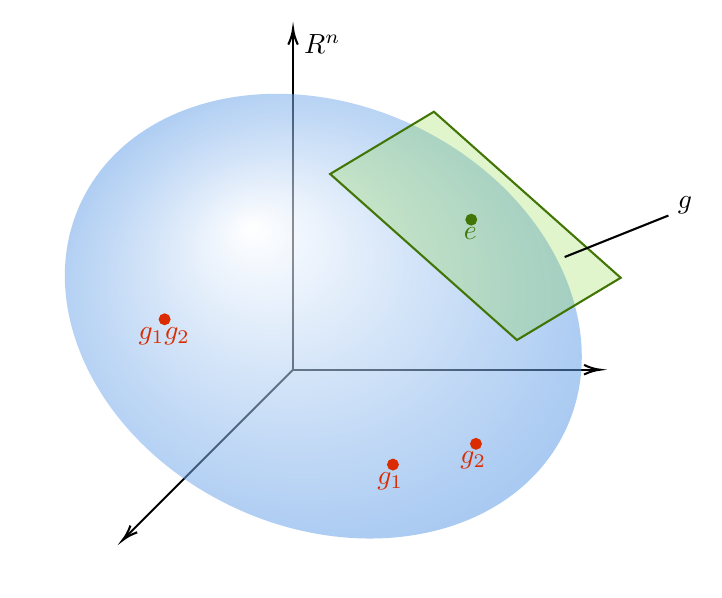
\begin{tikzpicture}[x=0.75pt,y=0.75pt,yscale=-1,xscale=1]
%uncomment if require: \path (0,300); %set diagram left start at 0, and has height of 300

%Straight Lines [id:da6341386319589457] 
\draw    (292.14,174.29) -- (292.14,12) ;
\draw [shift={(292.14,10)}, rotate = 90] [color={rgb, 255:red, 0; green, 0; blue, 0 }  ][line width=0.75]    (7.65,-2.3) .. controls (4.86,-0.97) and (2.31,-0.21) .. (0,0) .. controls (2.31,0.21) and (4.86,0.98) .. (7.65,2.3)   ;
%Straight Lines [id:da24449585878217006] 
\draw    (292.14,174.29) -- (438,174.29) ;
\draw [shift={(440,174.29)}, rotate = 180] [color={rgb, 255:red, 0; green, 0; blue, 0 }  ][line width=0.75]    (7.65,-2.3) .. controls (4.86,-0.97) and (2.31,-0.21) .. (0,0) .. controls (2.31,0.21) and (4.86,0.98) .. (7.65,2.3)   ;
%Straight Lines [id:da20393695102666232] 
\draw    (292.14,174.29) -- (211.41,255.01) ;
\draw [shift={(210,256.43)}, rotate = 315] [color={rgb, 255:red, 0; green, 0; blue, 0 }  ][line width=0.75]    (7.65,-2.3) .. controls (4.86,-0.97) and (2.31,-0.21) .. (0,0) .. controls (2.31,0.21) and (4.86,0.98) .. (7.65,2.3)   ;

%Shape: Donut [id:dp3968285728219174] 
\draw  [draw opacity=0][shading=_ahjd3yxh1,_rzlfkadph,path fading= _mgdafv76l ,fading transform={xshift=2}] (283.14,135.41) .. controls (283.14,135.41) and (293.7,141.26) .. (306.72,148.48) .. controls (319.74,155.7) and (330.3,161.55) .. (330.3,161.55) .. controls (330.3,161.55) and (319.74,155.7) .. (306.72,148.48) .. controls (293.7,141.26) and (283.14,135.41) .. (283.14,135.41)(194.07,86.04) .. controls (223.35,37.96) and (297.53,26.94) .. (359.75,61.43) .. controls (421.97,95.92) and (448.66,162.85) .. (419.37,210.93) .. controls (390.09,259) and (315.91,270.02) .. (253.69,235.53) .. controls (191.47,201.04) and (164.78,134.11) .. (194.07,86.04) ;
%Shape: Polygon [id:ds6798556831307849] 
\draw  [color={rgb, 255:red, 65; green, 117; blue, 5 }  ,draw opacity=1 ][fill={rgb, 255:red, 126; green, 211; blue, 33 }  ,fill opacity=0.23 ] (360,50) -- (450,130) -- (400,160) -- (310,80) -- cycle ;
%Straight Lines [id:da5149504674440749] 
\draw [color={rgb, 255:red, 65; green, 117; blue, 5 }  ,draw opacity=1 ]   (378,102) ;
\draw [shift={(378,102)}, rotate = 0] [color={rgb, 255:red, 65; green, 117; blue, 5 }  ,draw opacity=1 ][fill={rgb, 255:red, 65; green, 117; blue, 5 }  ,fill opacity=1 ][line width=0.75]      (0, 0) circle [x radius= 2.34, y radius= 2.34]   ;
%Straight Lines [id:da02432614019125645] 
\draw    (423,120) -- (473,100) ;
%Straight Lines [id:da40387644060361905] 
\draw [color={rgb, 255:red, 218; green, 44; blue, 0 }  ,draw opacity=1 ]   (340.26,220) ;
\draw [shift={(340.26,220)}, rotate = 0] [color={rgb, 255:red, 218; green, 44; blue, 0 }  ,draw opacity=1 ][fill={rgb, 255:red, 218; green, 44; blue, 0 }  ,fill opacity=1 ][line width=0.75]      (0, 0) circle [x radius= 2.34, y radius= 2.34]   ;
%Straight Lines [id:da3616646242174796] 
\draw [color={rgb, 255:red, 218; green, 44; blue, 0 }  ,draw opacity=1 ]   (380.26,210) ;
\draw [shift={(380.26,210)}, rotate = 0] [color={rgb, 255:red, 218; green, 44; blue, 0 }  ,draw opacity=1 ][fill={rgb, 255:red, 218; green, 44; blue, 0 }  ,fill opacity=1 ][line width=0.75]      (0, 0) circle [x radius= 2.34, y radius= 2.34]   ;
%Straight Lines [id:da10485113258612222] 
\draw [color={rgb, 255:red, 218; green, 44; blue, 0 }  ,draw opacity=1 ]   (230.26,150) ;
\draw [shift={(230.26,150)}, rotate = 0] [color={rgb, 255:red, 218; green, 44; blue, 0 }  ,draw opacity=1 ][fill={rgb, 255:red, 218; green, 44; blue, 0 }  ,fill opacity=1 ][line width=0.75]      (0, 0) circle [x radius= 2.34, y radius= 2.34]   ;

% Text Node
\draw (296,11.4) node [anchor=north west][inner sep=0.75pt]    {$\mathbb{R}^{n}$};
% Text Node
\draw (476,89.4) node [anchor=north west][inner sep=0.75pt]    {$\mathfrak{g}$};
% Text Node
\draw (373,104.4) node [anchor=north west][inner sep=0.75pt]  [color={rgb, 255:red, 65; green, 117; blue, 5 }  ,opacity=1 ]  {$e$};
% Text Node
\draw (331.26,222.4) node [anchor=north west][inner sep=0.75pt]  [color={rgb, 255:red, 218; green, 44; blue, 0 }  ,opacity=1 ]  {$g_{1}$};
% Text Node
\draw (371.26,212.4) node [anchor=north west][inner sep=0.75pt]  [color={rgb, 255:red, 218; green, 44; blue, 0 }  ,opacity=1 ]  {$g_{2}$};
% Text Node
\draw (216.26,152.4) node [anchor=north west][inner sep=0.75pt]  [color={rgb, 255:red, 218; green, 44; blue, 0 }  ,opacity=1 ]  {$g_{1} g_{2}$};

\end{tikzpicture}

    \caption{Visualization of the Lie Algebra}
    \label{fig:Lie Algebra}
\end{figure}
As seen in the figure, we have the manifold and group, which we denote $G$. We identify the identity element of this group, which we denote $e$.\endnote{The reason for this notation comes from the German origin of this word, where ``einheits'' means ``one''. Some other notations exist for the identity element but this is the most common.} We can recall from the Lie group that this identity is defined as an element of $G$ such that for all  $g \in G, e\cdot g=g\cdot e=g$. This identity element for matrix groups is simply the identity matrix, $\mathbb{I}(n)$. 

Once we have identified the identity element, we construct a `space' which is tangent to the manifold at that point. Since we know that the manifold must be differentiable, we are guaranteed to have a tangent space!

So this is the picture of the \gls{lie algebra}. We have a space that is tangent to the \gls{lie group} at the identity, and extends out. Since the \gls{lie algebra} is a flat space, it is much easier to work with than the curved surface of the manifold!

With the picture of the \gls{lie algebra} in mind, we can move to the formal definition. As before, I will lay out the formal definition and then break down the meaning. Before going straight into \glspl{lie algebra}, it is best to define what an \textit{algebra} is:
\begin{definition}[Algebra]
    An algebra, $\mathfrak{g}$, is a vector space over a field, $K$ with a multiplication, defined $*$, which is a binary operator, taking two inputs from $\mathfrak{g}$ and returning an output also in $\mathfrak{g}$. More succinctly, $\mathfrak{g}$ is an algebra if it is a vector space with a bilinear product.
\end{definition}
We have seen most of the elements of this definition before when discussing \glspl{lie group}. The notable feature here is that two inputs from $\mathfrak{g}$, when multiplied, are still in $\mathfrak{g}$. This is a feature that we call \textit{bilinearity}. We may denote this in standard notation as $\mathfrak{g}\times \mathfrak{g}\rightarrow \mathfrak{g}$.

We can formalize this definition of bilinearity to check if any operation is bilinear. If we denote $\mathfrak{g}$ as the vector space which $x,y$ and $z$ are elements of, and $a$ and $b$ as elements of $K$, then we have the following properties:
\begin{enumerate}
    \item Right Distributivity: $(x+y)\cdot z=x\cdot z+y\cdot z$
    \item Left Distributivity: $z\cdot(x+y)=z\cdot x +z\cdot y$
    \item Compatibility with scalars: $(ax)\cdot(by)=(ab)(x\cdot y)$
\end{enumerate}

\subsection{The Lie Bracket}
The particulars of algebras beyond this are not of great concern to us. Instead, we will be concerned with the specific properties of \glspl{lie algebra}. The \gls{lie algebra} is similar to an algebra, but has an additional operation. We define an operation called the \textit{Lie bracket}, which we denote $[\cdot,\cdot]$. We can think of the Lie bracket as a kind of weird multiplication. It takes two numbers from the algebra, and returns something else in the algebra.

For a \gls{lie algebra}, we must have the following properties for the Lie bracket. I introduce the notation $\forall x$ here which is shorthand for `for all $x$'.
\begin{itemize}
    \item It is bilinear (definition above)
    \item It is alternating, $[x,x]=0 \quad \forall x\in \mathfrak{g}$
    \item It is antisymmetric, meaning that $[x,y]=-[y,x] \ \forall x, y$
    \item It satisfies the Jacobi Identity, which states that: $[x,[y,z]]+[y,[z,x]]+[z,[x,y]]=0$.\endnote{Readers of Volume II should find there properties very similar to the properties of the wedge product. The \gls{lie algebra} and the Grassmann algebra over which the wedge product is defined are very similar.}
\end{itemize}

I should note that the property of being alternating and being skew-symmetric are the same.\endnote{\begin{proof}
    This can be proven by considering the identity from both directions to show equivalence. Both directions must be considered to show that the link is bijective. Starting with the antisymmetric property, we can substitute $y=x$. This gives us:
$$[x,x]=-[x,x]$$
The solution of which must be 0, since no other value satisfies this equality. 

From the other direction, we assume the alternating form $[x,x]=0 \ \forall x$. This can be equivalently applied on the expression:
$$[x+y,x+y]=0$$
The lie bracket is bilinear, so the terms can be expanded as follows:
$$[x,x]+[x,y]+[y,x]+[y,y]=0$$
From the assumption of the alternating form, $[x,x]$ and $[y,y]=0$. Thus,
$$[x,y]=-[y,x]$$
\end{proof}} In the future, it will suffice to show only one. Right now, this definition likely has no meaning to the reader. Let us consider the cross product as an example familiar to the reader:

\begin{example}[The cross product as a Lie bracket]
    We can start with the properties that we assumed for the \gls{lie algebra}. Taking the Lie bracket operation to be the cross product, that is: $[x,y]=x\times y$, it is easy to show that all of the properties are satisfied.

\textbf{Bilinearity:} taking $x$ and $y$ to be vectors, which we would commonly denote $\vec{x}$ and $\vec{y}$, we know that the cross product is defined when $x$ and $y$ exist in $\mathbb{R}^3$. We also know that the cross product generates a vector orthogonal to $x$ and $y$, which also exists in $\mathbb{R}^3$. So, we can see that the cross product satisfies bilinearity.

\textbf{Skew Symmetry:} It is commonly known that the cross product has the property that $x\times y=-y\times x$. This is commonly demonstrated with the right hand rule. Reversing the cross product direction flips the resultant direction.

We can show skew symmetry in another form though, using the matrix representation of the cross product. We can use two vectors, which we represent as follows:
$$\begin{pmatrix}
    a\\b\\c
\end{pmatrix} \times \begin{pmatrix}
    x\\y\\z
\end{pmatrix}$$
We have already shown that this should be a mapping from $\mathbb{R}^3\rightarrow\mathbb{R}^3$. If we take the matrix containing $a$, $b$, and $c$ to be fixed, we can represent it as a linear combination of $x$, $y$, and $z$. Performing the cross product, we can easily see how this is done:
$$\begin{pmatrix}
    a\\b\\c
\end{pmatrix} \times \begin{pmatrix}
    x\\y\\z
\end{pmatrix}=\begin{pmatrix}
    bz-cy\\cx-az\\ay-bx
\end{pmatrix}$$
So, we can simply rewrite the RHS as a matrix of $a$, $b$, and $c$:
$$\begin{pmatrix}
    0&-c&b\\c&0&-a\\-b&a&0
\end{pmatrix}\begin{pmatrix}
    x\\y\\z
\end{pmatrix}$$
So, we can see that the matrix for the cross product is also skew symmetric - but in a different way. For a matrix, we say that it is skew symmetric when $A^\top =-A$, which is shown in the matrix for the cross product. It turns out that this matrix \gls{lie algebra} is called $\mathfrak{so}(3)$ and is related to rotations, which we will investigate further later.

\textbf{Jacobi Identity:} Satisfaction of the Jacobi Identity is simply a practice of our algebraic skills, but it is still worthwhile to show that the cross product validates this identity for completeness. We can use the cross product shortcut to make this a bit easier:
$$ \overrightarrow{\underleftarrow{xyzxy}}$$
    The Jacobi Identity written as cross products gives us the following:
$$x\times(y\times z)+y\times (z\times x)+z \times (x\times y)=0$$
We can evaluate the expression in parenthesis first, giving:
$$x\times(x)+y\times (y)+z \times (z)=0$$
Since any vector crossed with itself is 0, the sum obviously goes to zero.\endnote{If you are uneasy with the shortcut method, an equivalent way to solve this problem is the use the triple scalar product identity:
$$A\times (B\times C) = B(A\cdot C)-C(A\cdot B)$$
Plugging this in to the Jacobi identity (and keeping in mind that the dot product is an commutative operation), we can see that this also gives us zero.} And so, we have shown that the cross product is a valid Lie bracket for $\mathbb{R}^3$.
\end{example}

\begin{exercise}
    We have shown previously that the \gls{lie algebra} can be written in a matrix form from \autoref{thm:Ado}. For matrices, we take the Lie bracket to be the \textit{commutator} of two matrices, which is defined
    $$[A,B]=AB-BA$$
    Show that the commutator as the Lie bracket produces a valid \gls{lie algebra}. You can follow the same steps as we did for the cross product. We will use the commutator heavily since we can define all Lie algebras in terms of matrices, so this is a good one to practice!
\end{exercise}

\section{Relating Lie Groups and Algebras}
In \autoref{sec:motivation and background lie}, I briefly discussed the \gls{exponential map} as a way to convert between the \gls{lie group} and the \gls{lie algebra}. Here, we will take that definition and solidify its meaning.

Up to now, we've developed this notion of groups and algebras. Our algebra is our simple definition, because everything there is our standard Euclidean geometry. We know our algebra looks like the group \textit{at} the identity because it is tangent. So, if we want to go from point A to point B, we can utilize the continuous structure to get there. Rotations, as we will later see, are a prototypical example of a \gls{lie group}. Therefore, we will understand the exponential map in this context.

Let's think briefly about doing a rotation by $\Theta$ degrees. Since we can only use our algebra, our `rule' is that we can only achieve this rotation using straight lines in our \gls{lie algebra}. So instead, of doing this rotation by $\Theta$, let's do a rotation by $\Theta/n$, $n$ times!\endnote{Choose $n$ in your head to be a really big number, like a zillion or so.} So, we can achieve this rotation by doing many, many small rotations, each of which look like straight lines. In the limit, each of these straight lines define the whole rotation. Let's call this small rotation $\theta\equiv\Theta/n$.

Let's put some exact math to this. We're going to use a bit of linear algebra now, but this is just to show how we arrive at the exponential map. We'll dive deeper into all of this understanding later. Given our initial location of point $P$ as $(x,y)$, we can define a coordinate transformation as in \autoref{fig:coord rot}.
\begin{figure}[ht]
    \centering



\tikzset{every picture/.style={line width=0.75pt}} %set default line width to 0.75pt        

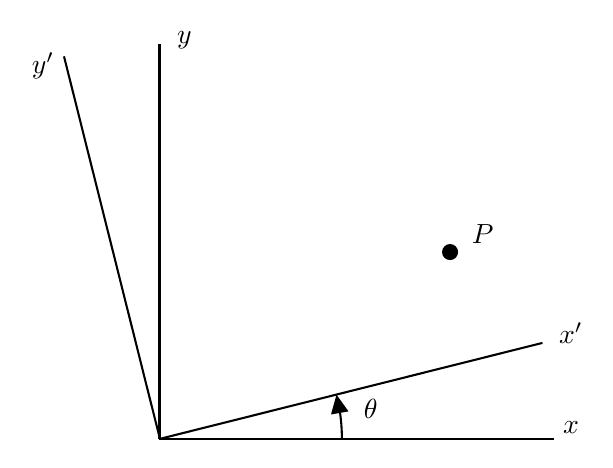
\begin{tikzpicture}[x=0.75pt,y=0.75pt,yscale=-1,xscale=1]
%uncomment if require: \path (0,300); %set diagram left start at 0, and has height of 300

%Straight Lines [id:da8667761635282387] 
\draw    (204,240) -- (394,240) ;
%Straight Lines [id:da5594582363385631] 
\draw    (204,240) -- (204,50) ;

%Straight Lines [id:da8791102017600835] 
\draw    (344,150) ;
\draw [shift={(344,150)}, rotate = 0] [color={rgb, 255:red, 0; green, 0; blue, 0 }  ][fill={rgb, 255:red, 0; green, 0; blue, 0 }  ][line width=0.75]      (0, 0) circle [x radius= 3.35, y radius= 3.35]   ;
%Straight Lines [id:da5043582166056578] 
\draw    (204.22,240) -- (388.51,193.78) ;
%Straight Lines [id:da9911097388256049] 
\draw    (204.22,240) -- (158,55.71) ;
%Shape: Arc [id:dp16728017926039918] 
\draw  [draw opacity=0] (289.3,218.73) .. controls (290.99,225.54) and (291.89,232.67) .. (291.89,240) -- (204,240) -- cycle ; \draw    (289.98,221.71) .. controls (291.23,227.61) and (291.89,233.73) .. (291.89,240) ;  \draw [shift={(289.3,218.73)}, rotate = 80] [fill={rgb, 255:red, 0; green, 0; blue, 0 }  ][line width=0.08]  [draw opacity=0] (8.93,-4.29) -- (0,0) -- (8.93,4.29) -- cycle    ;

% Text Node
\draw (397,230.4) node [anchor=north west][inner sep=0.75pt]    {$x$};
% Text Node
\draw (211,42.4) node [anchor=north west][inner sep=0.75pt]    {$y$};
% Text Node
\draw (395,182.4) node [anchor=north west][inner sep=0.75pt]    {$x'$};
% Text Node
\draw (141,52.4) node [anchor=north west][inner sep=0.75pt]    {$y'$};
% Text Node
\draw (301,219.4) node [anchor=north west][inner sep=0.75pt]    {$\theta $};
% Text Node
\draw (353,135.4) node [anchor=north west][inner sep=0.75pt]    {$P$};

\end{tikzpicture}
    
    \caption{Rotation of coordinate system}
    \label{fig:coord rot}
\end{figure}

From simple geometry, it is evident that in our new coordinate system, we may express the point $P$ as:
\begin{gather}
    x'=x\cos\theta+y\sin\theta\\
    y'=-x\sin\theta+y\cos\theta
\end{gather}
These trigonometric functions are no good for our straight line version. We can represent the infinitesimal rotation \textit{exactly} with the first derivative:
\begin{gather}
    x'=x+y\theta\\
    y'=-x\theta+y
\end{gather}
Let's put this into a matrix form now:
$$\begin{bmatrix}
    x'\\y'
\end{bmatrix}=\begin{bmatrix}
    1&\theta\\-\theta&1
\end{bmatrix}\begin{bmatrix}
    x\\y
\end{bmatrix}$$
We now have a mapping that tells us how exactly an infinitesimal transformation takes us from the $x,y$ coordinates into the $x',y'$ coordinates. Notice, \textit{everything} in this equation is linear when we consider this infinitesimal $\theta$.

Let's notice that part of our answer is the identity matrix, $I$. Let's pull that component out from this equation, so that we have:
$$\begin{bmatrix}
    1&\theta\\-\theta&1
\end{bmatrix}=\begin{bmatrix}
    1&0\\0&1
\end{bmatrix}+\begin{bmatrix}
    0&\theta\\-\theta&0
\end{bmatrix}$$
Let's go ahead and denote all of these matrices symbolically to make our math look a bit nicer. Our LHS matrix we'll call $R(\theta)$ -- this is our matrix which represents a coordinate transformation by some small $\theta$. On the right hand side, we have our identity, $\mathbb{I}$. This identity part is present because it's the `do nothing' part of our rotation. It is what's preserving what we already have, in a sense. We also have our matrix of $\theta$ values. This matrix is what is actually causing some change in the object. We're going to give this one a special name, $\mathcal{J}$, which we call a \textit{generator matrix}, since it is what is generating our rotation (by convention, we will factor our the $\theta$ so that our generator matrix is just the coefficients). With our new symbols, we can write the equation above again:
$$R(\theta)=\mathbb{I}+\theta\mathcal{J}$$
Now, we can finally appreciate how we get from the \gls{lie algebra} to the \gls{lie group}. Right now, we are considering a infinitesimal rotation $\theta$. Let's remember our original premise, though: We split our full rotation into $n$ pieces, and multiply all those $\Theta/n$ rotations together. Why do we multiply? Because this rotation is a group, and multiplication of two group elements yields a third element guaranteed to also be in the group. Mathematically:
$$R(\Theta)=\left(R(\theta)\right)^n=\left(\mathbb{I}+\theta\mathcal{J}\right)^n$$
Let's remember that $\theta\equiv\Theta/n$. Plugging this into our formula, we get our final result:
$$R(\Theta)=\left(\mathbb{I}+\frac{\Theta}{n}\mathcal{J}\right)^n$$
This formula should hopefully be familiar! This is exactly reminiscent to how we define the exponential operation:
$$e^x=\lim_{n\rightarrow\infty}{\left(1+\frac{x}{n}\right)^n}$$
This is, at the core, \textit{why} our exponential map is what takes us from the \gls{lie algebra} to the \gls{lie group}. The repeated multiplication of many small linear groups is \textit{exactly} the same as our exponential function.

Notice that we only required the first derivative of our function to construct this very powerful representation of the group. In fact, we constructed our generator by considering the derivative at the identity:
$$\mathcal{J}=\frac{dR(\Theta)}{d\Theta}\Biggr\rvert_{\Theta=0}$$
You should notice a great parallel here in how we constructed our \gls{lie algebra}.

\subsection{Exponential Maps}

Our \gls{lie algebra}, in general, is not going to be a real number. As we saw with the cross product and the coordinate transformation, it is often a matrix or complex number instead. As we say earlier from \autoref{thm:Ado}, we may in fact represent almost any \gls{lie group} or 
\gls{lie algebra} with a matrix.

Although we have shown above that the exponential allows us to go from the \gls{lie algebra} to the \gls{lie group}, there is still a question of what exactly our exponential operation will look like for these objects. It seems that it will vary depending on our representation. How can we find a general exponential for these?

To do this, we turn to the Taylor expansion of $e^x$ for an answer. We can write the Taylor expansion as a summation:
\begin{equation}\label{eq:taylor exp}
    e^x\equiv\sum_{n=0}^\infty{\frac{x^n}{n!}}
\end{equation}

This is the definition that we use for many the more complicated cases, such as complex numbers and matrices. Since we are only using integer indices for $n$, all of these operations are well-defined and valid.

\begin{exercise}
    Use the definition of the exponential as a Taylor series as shown in \eqautoref{eq:taylor exp} to write a closed form for the complex exponential, $e^{i\theta}$. It will be helpful to know / look up the Taylor series for $\sin\theta$ and $\cos\theta$.
\end{exercise}

So, we have a way to write any arbitrary exponential. We can then use this exponential, which we will call the \textit{exponential map}, to convert from the \gls{lie algebra} to the \gls{lie group}. We write this as:
$$\exp:\mathfrak{g}\rightarrow G$$
As we have noted before, this is useful because we can do operations on $\mathfrak{g}$, which is generally simpler to describe since it is a vector space, and then use the exponential map to put this back on to the manifold!

Heretofor, we will mostly use matrix representations for our \glspl{lie group} and \glspl{lie algebra}. Therefore, I have included \autoref{sec: computation of matrix exp} which covers the variety of methods for the computation of matrix exponentials.

\section{Bringing it Together - The Circle Group}
Let's bring all of the previously mentioned concepts of \gls{lie theory} together into one concrete example. This example will showcase the full process of describing the \gls{lie group}, \gls{lie algebra}, and \gls{exponential map}. The prototypical example of study here is the circle group. Since most of us have been studying circles since preschool, this should be a fairly interesting example!

We'll start by describing the group itself. We often call this group $\mathbb{S}^1$, which is a very fancy way of saying the group is a circle. $S$ refers to spheres, and the superscript to the dimension. $S^0$ is a point, $S^1$ to circles, $S^2$ to the surface of a sphere, and so on. The $\mathbb{S}$ is used to distinguish the group from the surface itself.

To actually define the group, we want to construct the unit circle. We know the unit circle has a magnitude of 1 everywhere. So, we know the group must be composed of all complex numbers with magnitude 1. We can then write the circle group:
$$\mathbb{S}^1=\{z\in\mathbb{C}:|z|=1\}$$
 We know from the name that this is a group, but let's go ahead and prove it anyways -- we won't always know if the set that we've constructed is a group.
\subsubsection{Group Characteristics of $\mathbb{S}^1$}
\begin{enumerate}
    \item Closure: for all $z$ satisfying the conditions of $\mathbb{S}^1$, we can show that the result must also be in $\mathbb{S}^1$. We can compose any complex number $z$ as it's magnitude $r$, and direction, $\theta$, as $re^{i\theta}$. Taking any two elements of $\mathbb{S}^1$, the multiplication is $r_1e^{i\theta_1}\cdot r_2e^{i\theta_2}=r_1r_2e^{i(\theta_1+\theta_2)}$. Since the magnitude $r$ must be 1 for any element of $\mathbb{S}^1$, the product must also be an element in $\mathbb{S}^1$.
    \item Complex multiplication is known to be associative. Since $\mathbb{S}^1\subset\mathbb{C}$, it must also be associative under multiplication.
    \item The identity element for complex numbers is $1+0i$. This has a magnitude of 1 so it is part of $\mathbb{S}^1$.
    \item The inverse of a complex number is defined as $$z^{-1}\equiv\frac{\bar{z}}{z\bar{z}}$$
Where $\bar{z}$ is the complex conjugate of $z$. If $z=\sigma+i\omega$, the complex conjugate $\bar{z}=\sigma-i\omega$. We can use the properties described when discussing closure to show that both $z$ and $\bar{z}$ have magnitude 1. Thus, the inverse is also a part of the circle group.
\end{enumerate}

So, with all four axioms satisfied, we have shown that $\mathbb{S}^1$ is indeed a group! Although we will not prove it precisely, we can also see that the circle group is also a manifold - there are no discontinuities on the circle. So, the circle group defines a \gls{lie group}!

\subsubsection{Algebraic Characteristics of $\mathbb{S}^1$}
Now that we have identified the identity element of $\mathbb{S}^1$, we can construct its algebra. We'll start with a depiction of the group first, which is shown in \autoref{fig:circle group}.
\begin{figure}[ht]
    \centering


\tikzset{every picture/.style={line width=0.75pt}} %set default line width to 0.75pt        

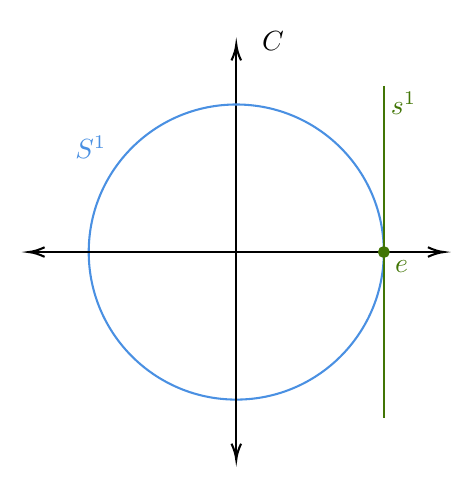
\begin{tikzpicture}[x=0.75pt,y=0.75pt,yscale=-1,xscale=1]
%uncomment if require: \path (0,300); %set diagram left start at 0, and has height of 300

%Straight Lines [id:da7075691361286388] 
\draw    (290,150) -- (290,52) ;
\draw [shift={(290,50)}, rotate = 90] [color={rgb, 255:red, 0; green, 0; blue, 0 }  ][line width=0.75]    (7.65,-2.3) .. controls (4.86,-0.97) and (2.31,-0.21) .. (0,0) .. controls (2.31,0.21) and (4.86,0.98) .. (7.65,2.3)   ;
%Straight Lines [id:da8934579482018679] 
\draw    (290,150) -- (388,150) ;
\draw [shift={(390,150)}, rotate = 180] [color={rgb, 255:red, 0; green, 0; blue, 0 }  ][line width=0.75]    (7.65,-2.3) .. controls (4.86,-0.97) and (2.31,-0.21) .. (0,0) .. controls (2.31,0.21) and (4.86,0.98) .. (7.65,2.3)   ;
%Shape: Circle [id:dp5981456072784835] 
\draw  [color={rgb, 255:red, 74; green, 144; blue, 226 }  ,draw opacity=1 ] (218.91,150) .. controls (218.91,110.74) and (250.74,78.91) .. (290,78.91) .. controls (329.26,78.91) and (361.09,110.74) .. (361.09,150) .. controls (361.09,189.26) and (329.26,221.09) .. (290,221.09) .. controls (250.74,221.09) and (218.91,189.26) .. (218.91,150) -- cycle ;
%Straight Lines [id:da7438012851289106] 
\draw    (290,150) -- (192,150) ;
\draw [shift={(190,150)}, rotate = 360] [color={rgb, 255:red, 0; green, 0; blue, 0 }  ][line width=0.75]    (7.65,-2.3) .. controls (4.86,-0.97) and (2.31,-0.21) .. (0,0) .. controls (2.31,0.21) and (4.86,0.98) .. (7.65,2.3)   ;
%Straight Lines [id:da24761338831710056] 
\draw    (290,150) -- (290,248) ;
\draw [shift={(290,250)}, rotate = 270] [color={rgb, 255:red, 0; green, 0; blue, 0 }  ][line width=0.75]    (7.65,-2.3) .. controls (4.86,-0.97) and (2.31,-0.21) .. (0,0) .. controls (2.31,0.21) and (4.86,0.98) .. (7.65,2.3)   ;
%Straight Lines [id:da7580332264955227] 
\draw [color={rgb, 255:red, 65; green, 117; blue, 5 }  ,draw opacity=1 ]   (361,70) -- (361,230) ;
%Straight Lines [id:da4429390842170522] 
\draw [color={rgb, 255:red, 65; green, 117; blue, 5 }  ,draw opacity=1 ]   (361.09,150) ;
\draw [shift={(361.09,150)}, rotate = 0] [color={rgb, 255:red, 65; green, 117; blue, 5 }  ,draw opacity=1 ][fill={rgb, 255:red, 65; green, 117; blue, 5 }  ,fill opacity=1 ][line width=0.75]      (0, 0) circle [x radius= 2.34, y radius= 2.34]   ;

% Text Node
\draw (301,42.4) node [anchor=north west][inner sep=0.75pt]    {$\mathbb{C}$};
% Text Node
\draw (365,152.4) node [anchor=north west][inner sep=0.75pt]  [color={rgb, 255:red, 65; green, 117; blue, 5 }  ,opacity=1 ]  {$e$};
% Text Node
\draw (211,92.4) node [anchor=north west][inner sep=0.75pt]  [color={rgb, 255:red, 74; green, 144; blue, 226 }  ,opacity=1 ]  {$\mathbb{S}^{1}$};
% Text Node
\draw (363,71.4) node [anchor=north west][inner sep=0.75pt]  [color={rgb, 255:red, 65; green, 117; blue, 5 }  ,opacity=1 ]  {$\mathfrak{s}^{1}$};

\end{tikzpicture}

    \caption{The Circle Group as a Lie group and algebra}
    \label{fig:circle group}
\end{figure}

We notice the identity element at $1+0i$ which is denoted $e$. We construct the tangent to the identity to form the \gls{lie algebra}, which is denoted $\mathfrak{s}^1$. This line forms the \gls{lie algebra} of the circle group. Now, we can construct vectors on the \gls{lie algebra}. Since the algebra $\mathfrak{s}^1$ is a vertical line, the vectors we construct will be purely imaginary. So we can write these vectors as $i\theta$, where $\theta \in \mathbb{R}$ is some arbitrary constant which describes the length of the vector.

Our Lie bracket for this case is trivial. Since multiplication over $\mathbb{R}$ is commutative, the only way for $[\theta_1,\theta_2]=-[\theta_1,\theta_2]$ is if the Lie bracket operation is 0.

\subsubsection{The Exponential Map of the Circle Group}
The last thing to do is to describe the \gls{lie group} $\mathbb{S}^1$ in terms of the \gls{lie algebra} $\mathfrak{s}^1$. We can write this exponential map as:
$$\exp:\mathfrak{s}^1\rightarrow\mathbb{S}^1$$
Since the elements of $\mathfrak{s}^1$ are purely imaginary, the exponential map is the complex exponential. So we have $e^{i\theta}$ as the exponential map for the vector $i\theta$ in the \gls{lie algebra}. We show this diagrammatically in \autoref{fig:circ exp map}.

\begin{figure}[ht]
    \centering


\tikzset{every picture/.style={line width=0.75pt}} %set default line width to 0.75pt        

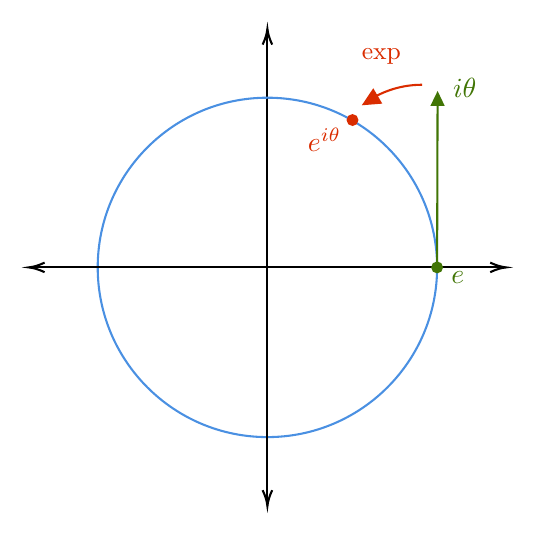
\begin{tikzpicture}[x=0.75pt,y=0.75pt,yscale=-1,xscale=1]
%uncomment if require: \path (0,300); %set diagram left start at 0, and has height of 300

%Straight Lines [id:da4874941140341892] 
\draw    (265,135) -- (265,22) ;
\draw [shift={(265,20)}, rotate = 90] [color={rgb, 255:red, 0; green, 0; blue, 0 }  ][line width=0.75]    (7.65,-2.3) .. controls (4.86,-0.97) and (2.31,-0.21) .. (0,0) .. controls (2.31,0.21) and (4.86,0.98) .. (7.65,2.3)   ;
%Straight Lines [id:da22303785560441036] 
\draw    (265,135) -- (378,135) ;
\draw [shift={(380,135)}, rotate = 180] [color={rgb, 255:red, 0; green, 0; blue, 0 }  ][line width=0.75]    (7.65,-2.3) .. controls (4.86,-0.97) and (2.31,-0.21) .. (0,0) .. controls (2.31,0.21) and (4.86,0.98) .. (7.65,2.3)   ;
%Shape: Ellipse [id:dp7593851313048715] 
\draw  [color={rgb, 255:red, 74; green, 144; blue, 226 }  ,draw opacity=1 ] (183.24,135) .. controls (183.24,89.85) and (219.85,53.24) .. (265,53.24) .. controls (310.15,53.24) and (346.76,89.85) .. (346.76,135) .. controls (346.76,180.15) and (310.15,216.76) .. (265,216.76) .. controls (219.85,216.76) and (183.24,180.15) .. (183.24,135) -- cycle ;
%Straight Lines [id:da870819452925987] 
\draw    (265,135) -- (152,135) ;
\draw [shift={(150,135)}, rotate = 360] [color={rgb, 255:red, 0; green, 0; blue, 0 }  ][line width=0.75]    (7.65,-2.3) .. controls (4.86,-0.97) and (2.31,-0.21) .. (0,0) .. controls (2.31,0.21) and (4.86,0.98) .. (7.65,2.3)   ;
%Straight Lines [id:da16757460890379539] 
\draw    (265,135) -- (265,248) ;
\draw [shift={(265,250)}, rotate = 270] [color={rgb, 255:red, 0; green, 0; blue, 0 }  ][line width=0.75]    (7.65,-2.3) .. controls (4.86,-0.97) and (2.31,-0.21) .. (0,0) .. controls (2.31,0.21) and (4.86,0.98) .. (7.65,2.3)   ;
%Straight Lines [id:da42905597551393193] 
\draw [color={rgb, 255:red, 65; green, 117; blue, 5 }  ,draw opacity=1 ]   (346.76,135) ;
\draw [shift={(346.76,135)}, rotate = 0] [color={rgb, 255:red, 65; green, 117; blue, 5 }  ,draw opacity=1 ][fill={rgb, 255:red, 65; green, 117; blue, 5 }  ,fill opacity=1 ][line width=0.75]      (0, 0) circle [x radius= 2.34, y radius= 2.34]   ;
%Straight Lines [id:da27239627369242314] 
\draw [color={rgb, 255:red, 65; green, 117; blue, 5 }  ,draw opacity=1 ]   (346.76,135) -- (346.99,53) ;
\draw [shift={(347,50)}, rotate = 90.16] [fill={rgb, 255:red, 65; green, 117; blue, 5 }  ,fill opacity=1 ][line width=0.08]  [draw opacity=0] (7.14,-3.43) -- (0,0) -- (7.14,3.43) -- cycle    ;
%Straight Lines [id:da9820046812940839] 
\draw [color={rgb, 255:red, 218; green, 44; blue, 0 }  ,draw opacity=1 ]   (306,64) ;
\draw [shift={(306,64)}, rotate = 0] [color={rgb, 255:red, 218; green, 44; blue, 0 }  ,draw opacity=1 ][fill={rgb, 255:red, 218; green, 44; blue, 0 }  ,fill opacity=1 ][line width=0.75]      (0, 0) circle [x radius= 2.34, y radius= 2.34]   ;
%Shape: Arc [id:dp7703254831753583] 
\draw  [draw opacity=0] (310.47,56.9) .. controls (318.5,50.69) and (328.57,47) .. (339.5,47) -- (339.5,94.5) -- cycle ; \draw [color={rgb, 255:red, 218; green, 44; blue, 0 }  ,draw opacity=1 ]   (312.94,55.11) .. controls (320.52,49.99) and (329.66,47) .. (339.5,47) ;  \draw [shift={(310.47,56.9)}, rotate = 329.63] [fill={rgb, 255:red, 218; green, 44; blue, 0 }  ,fill opacity=1 ][line width=0.08]  [draw opacity=0] (8.93,-4.29) -- (0,0) -- (8.93,4.29) -- cycle    ;

% Text Node
\draw (352.15,135.45) node [anchor=north west][inner sep=0.75pt]  [color={rgb, 255:red, 65; green, 117; blue, 5 }  ,opacity=1 ]  {$e$};
% Text Node
\draw (353,42.4) node [anchor=north west][inner sep=0.75pt]  [font=\normalsize,color={rgb, 255:red, 65; green, 117; blue, 5 }  ,opacity=1 ]  {$i\theta $};
% Text Node
\draw (283,66.4) node [anchor=north west][inner sep=0.75pt]  [color={rgb, 255:red, 218; green, 44; blue, 0 }  ,opacity=1 ]  {$e^{i\theta }$};
% Text Node
\draw (309,28.4) node [anchor=north west][inner sep=0.75pt]  [font=\small,color={rgb, 255:red, 218; green, 44; blue, 0 }  ,opacity=1 ]  {$\exp$};


\end{tikzpicture}

    
    \caption{Circle Group Exponential Map}
    \label{fig:circ exp map}
\end{figure}

When we think about it, this exponential map is quite amazing! It takes a vector which is along a straight line and `bends' it onto the circle! And from this result, we get a sort of intuition for why $e^{i\theta}$ describes the unit circle. All of this is very exciting, but we can further extend this by considering the matrix representation of this group.
\subsubsection{The Circle Group with Matrices}
We can equivalently represent the circle group with matrices. \
\cite{crawford_complex_2022} has a good overview of how we can construct a $2{\times}2$  matrix that represents the complex numbers. We will explore a version of the derivation here.

The basic problem when converting the circle group to a matrix representation is preserving all of the properties that the original circle group has. We call such a preservation of properties an \textit{isomorphism}. In the circle group, we represented our elements with the complex numbers, which are of form $\sigma+i\omega$. Our goal is to find a set of matrices that are \textit{isomorphic} to these complex numbers.

We have two axes in the complex plane, so we naturally choose $2{\times}2$ matrices as our basis of choice. The real part of the number is easy to describe. We know that any real number $a$ multiplied by 1 is just $a$. We call $1$ the multiplicative identity for this reason. For a matrix $A$, the corresponding action is to multiply by the identity, $\mathbb{I}$. So we can see that $\mathbb{I}$ is analogous to the number 1. So we can represent every real number $\sigma$ as $$\sigma\cdot\mathbb{I}=\begin{bmatrix}
    \sigma&0\\0&\sigma
\end{bmatrix},\ \sigma\in\mathbb{R}$$
The imaginary part is a bit more complicated, but we can take a systematic approach to find an appropriate matrix representation. Of course, we know that $i^2=-1$. So we should analogously find a matrix $A$ for the complex numbers such that $A^2=-\mathbb{I}$. We can use this equation to shed light on the values of the matrix $A$:

\begin{gather}
    A=\begin{bmatrix}
    a&b\\c&d
\end{bmatrix}\\
A^2=\begin{bmatrix}
    a&b\\c&d
\end{bmatrix}\begin{bmatrix}
    a&b\\c&d
\end{bmatrix}=\begin{bmatrix}
    a^2+bc&ab+bd\\ac+cd&bc+d^2
\end{bmatrix}
\end{gather}
Setting this equal to $-\mathbb{I}$, we have the following four conditions:
\begin{gather}
    a^2+bc=-1\\
    ab+bd=0\\
    ac+cd=0\\
    bc+d^2=-1
\end{gather}

We also know that $|i|=1$, which gives us another condition. For a matrix, the analogue of the magnitude is the determinant, the reasoning for which I describe briefly in \autoref{sec:role of the determinant}. This gives us $\det A=1$, yielding a final equation, $ad-bc=1$.

Even though it \textit{looks} like we should be able to solve this system of 4 variables with 5 equations, we actually have some redundant conditions which means that three solutions are possible here. There are two ways out of this predicament: we can either use some properties of rotations that are known (that the matrices are orthogonal, which we will discuss later) or we can assume that the values of the matrix must be real numbers.

The first option is circular reasoning (no pun intended) since we need to understand this group before we could apply this property, so we opt for the second option. It turns out that there is only one possible solution such that ($\ni$) $ a,b,c,d\in \mathbb{R}$.

That solution is given by $$A=\begin{bmatrix}
    0&-1\\1&0
\end{bmatrix}$$
Notice that this $A$ matrix is the exact same as the generator matrix, $\mathcal{J}$, which we created previously. Altogether, we have successfully constructed a real and imaginary number using matrices. To summarize, we can write the matrix equivalent of an imaginary number and then write a matrix of the form:
$$\Re(z)\begin{bmatrix}
    1&0\\0&1
\end{bmatrix}+\Im(z)\begin{bmatrix}
    0&-1\\1&0
\end{bmatrix},z=\begin{bmatrix}
    \Re(z)&-\Im(z)\\\Im(z)&\Re(z)
\end{bmatrix}$$
Now that we have constructed this matrix representation, we can return to the purpose of finding the \gls{lie group} and \gls{lie algebra}.

Our identity element is easy to identify, it is simply $\mathbb{I}$. Let's remember that our \gls{lie algebra} was identified as the purely complex components, or the matrix:
$$A=\mathcal{J}=\begin{bmatrix}
    0&-1\\1&0
\end{bmatrix}$$
We have the imaginary matrix $A$, and some arbitrary length of that vector, $\theta$. We can then map this on to the circle group with the matrix exponential:
$$e^{A\theta}=\exp\left(\begin{bmatrix}
    0&-\theta\\\theta&0
\end{bmatrix}\right)$$
Performing any of the methods for finding the matrix exponential, we find that the final matrix is:
$$\begin{bmatrix}
    \cos\theta&-\sin\theta\\\sin\theta&\cos\theta
\end{bmatrix}$$
We have recovered a rotation matrix as a result! This is a very exciting result. We have shown that we can understand rotations in the context of \gls{lie theory}. 

Before we move on, let's notice something else interesting about this matrix representation. If we consider the eigenvalues of $\theta \mathcal{J}$, we have:
$$\begin{vmatrix}
    -\lambda&-\theta\\\theta&-\lambda
\end{vmatrix}=0$$
Computing this determinant, we find that the eigenvalues of the generator matrix are $\pm i\theta $. It is apparent that these eigenvalues are the same as the \gls{lie algebra} which had found before, when we derived the circle group geometrically. Interestingly, we may directly compute the exponential of these eigenvalues to get the expression of the \gls{lie group}:
$$e^\lambda=e^{\pm i\theta}$$
These results show us that the matrix representation can recover the same information as our geometric interpretation. From here, it is useful to spend some more time looking deeply at rotation groups and other useful \glspl{lie group} to determine properties which benefit us in engineering and physics contexts.
\newpage
\printendnotes

\chapter{The Implications of Lie Theory}
After laying out some fundamentals of \gls{lie theory}, we can start applying it to actual problems we encounter to see how we can use it in aerospace and physics applications. These applications, especially in physics, are very numerous. Here, we will focus on the applications which are especially important to rotations, differential equations, and control theory. A brief aside on the uses in physics will be presented at the end. With some practical knowledge attained, we may begin exploring the use in control theory.

\section{Rotations}
We've started to discuss rotations with the circle group, but we will now expand that to include information on more general rotations and some of the other attributes.

Volume II has extensive information on rotations, but it will be helpful to solidify that information with the mathematics of \glspl{lie group}. Additionally, this means that we can gain an understanding of \textit{any possible} implementation of rotation schemes, because this underlying principle dictates all of them.

We can start with an example you can try at home to whet our appetite for the math to come.

\begin{example}[Infinitesimal Rotations]
    We can demonstrate the application of \gls{lie theory} to rotations in the real world fairly easily.  We know from Volume I and Volume II that two different rotation sequences -- say 3-2-1 and 3-1-3 -- will yield different results when we rotate through the same angle using each. That is to say, rotations are not generally commutative. The order in which perform these operations will change the final output.

    We can show this fairly easily in real life! We can take any object which has 3 distinct axes that are easily distinguishable -- a book or phone, as an example -- and rotate them according to each sequence.

    In fact, your head is another good example! Most of our necks are not especially flexible (to rotate in the magnitudes we need, at least). However we naturally associate motions of `pitch', `roll' and `yaw' with different head movements so it's quite an intuitive one to use for rotations.

    When we perform large rotations, such as rotating our object through each axis by $90\degree$, we very obviously get different final orientations. I demonstrate this in \autoref{fig:large rot}.

    \begin{figure}[H]
        \centering
        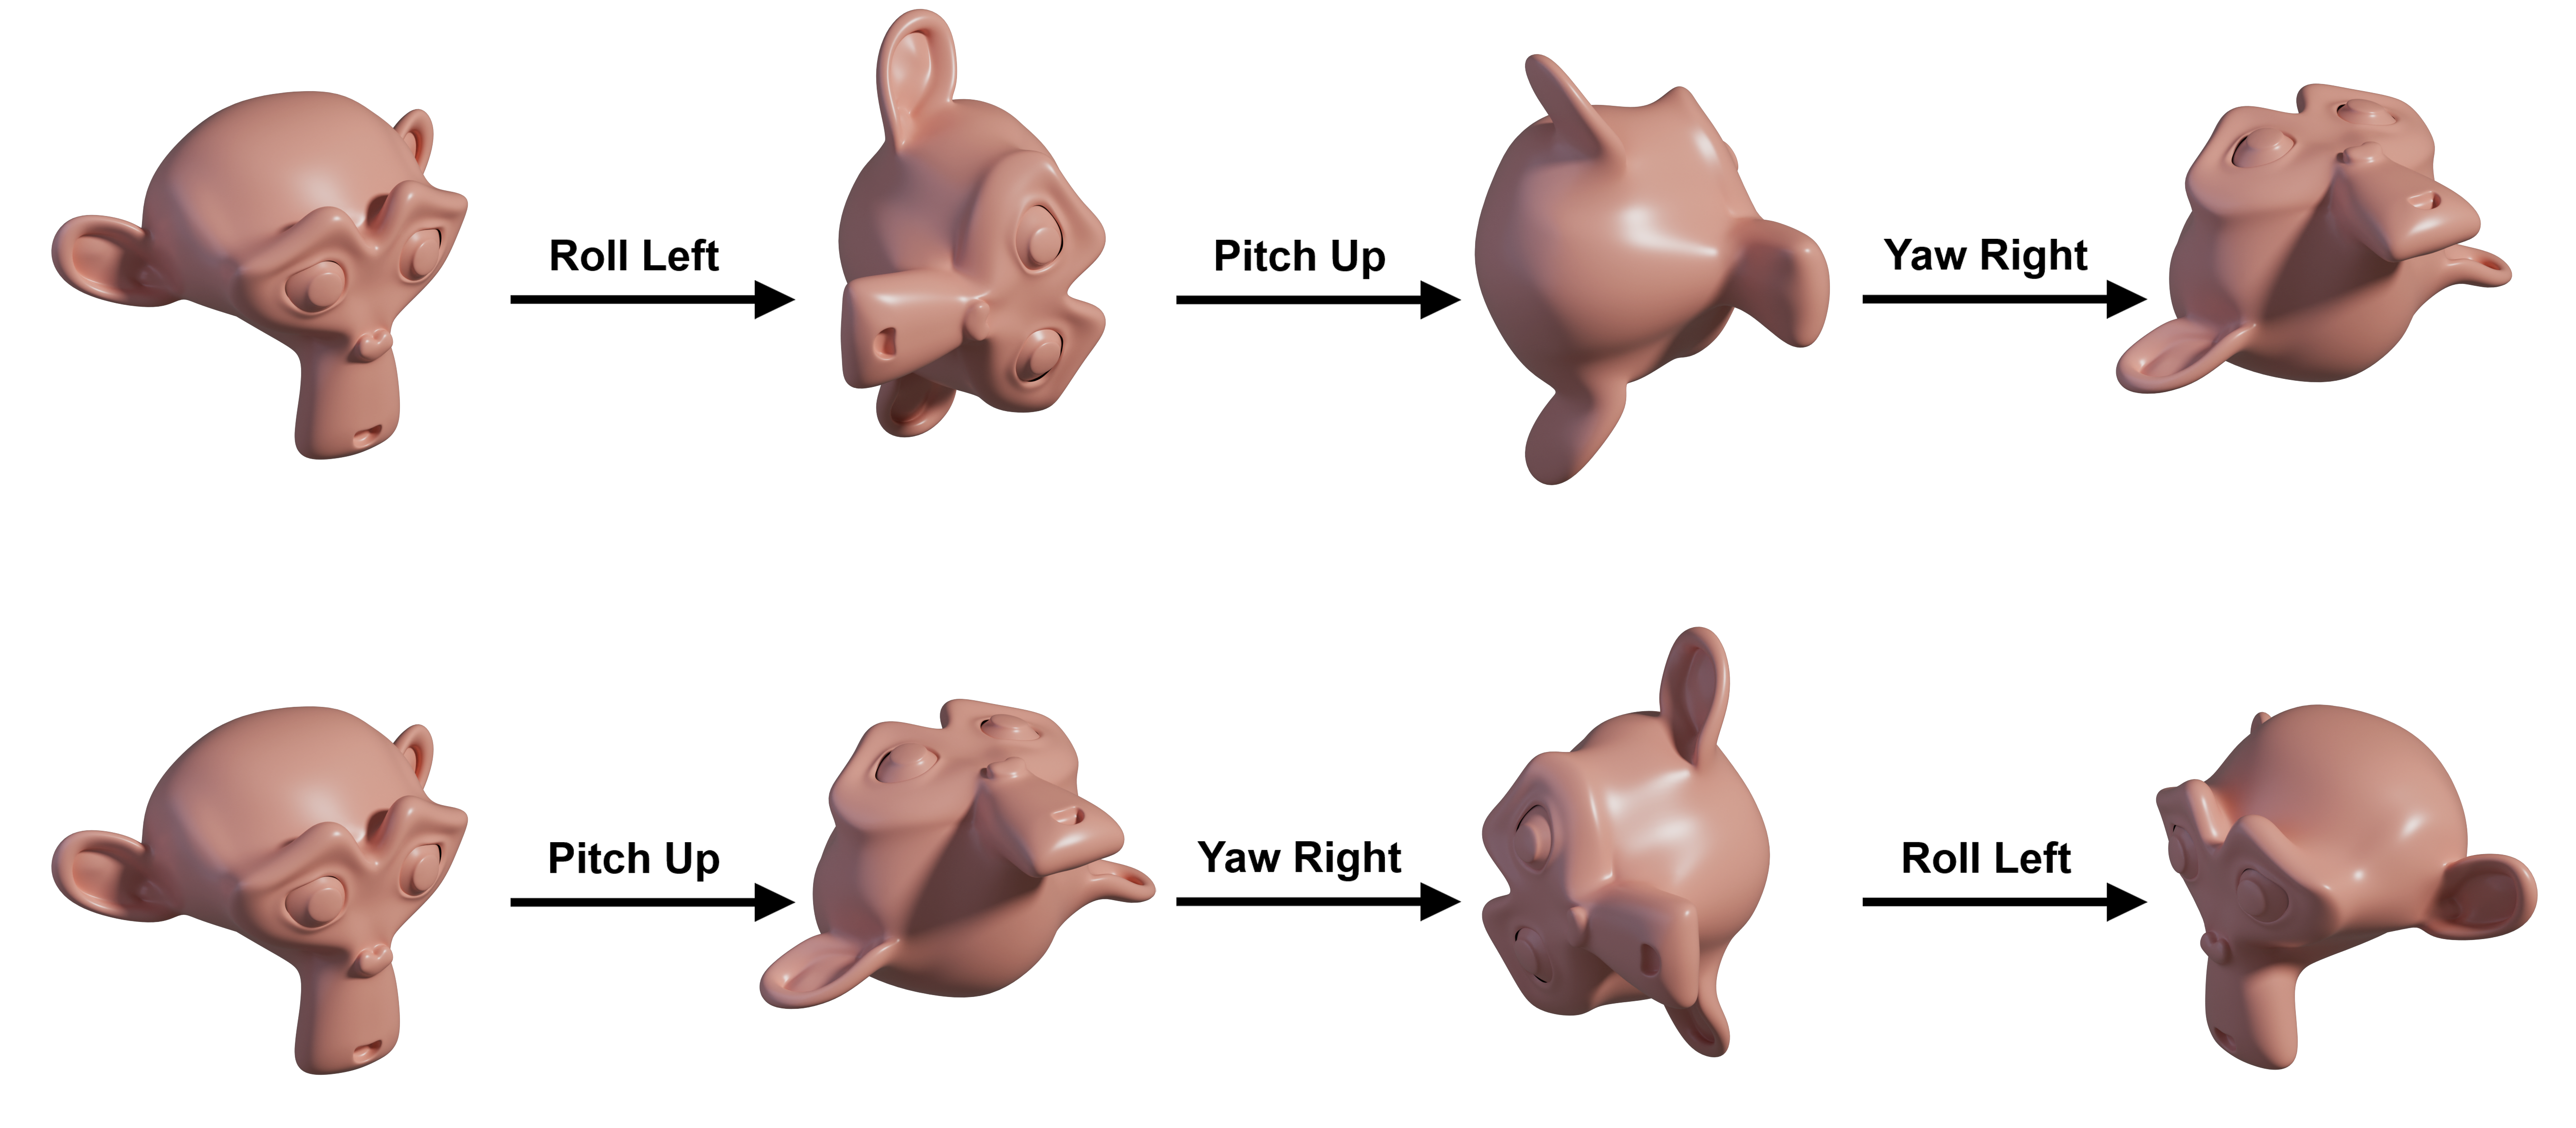
\includegraphics[width=\linewidth]{Images/LargeRotationsExample.png}
        \caption{Example of non-commutative rotation sequences}
        \label{fig:large rot}
    \end{figure}
    As we can see, our monkey, Suzanne, has ended up in very different rotations in either case, even though we performed the same rotation operations. Of course, if you have read Volume II, this is not at all an unexpected result. 

However, something interesting happens if we consider rotations that are small in magnitude. This is best shown visually, which we will do in \autoref{fig:small rot}. Each rotation in this image is only $10\degree$.

\begin{figure}[H]
    \centering
    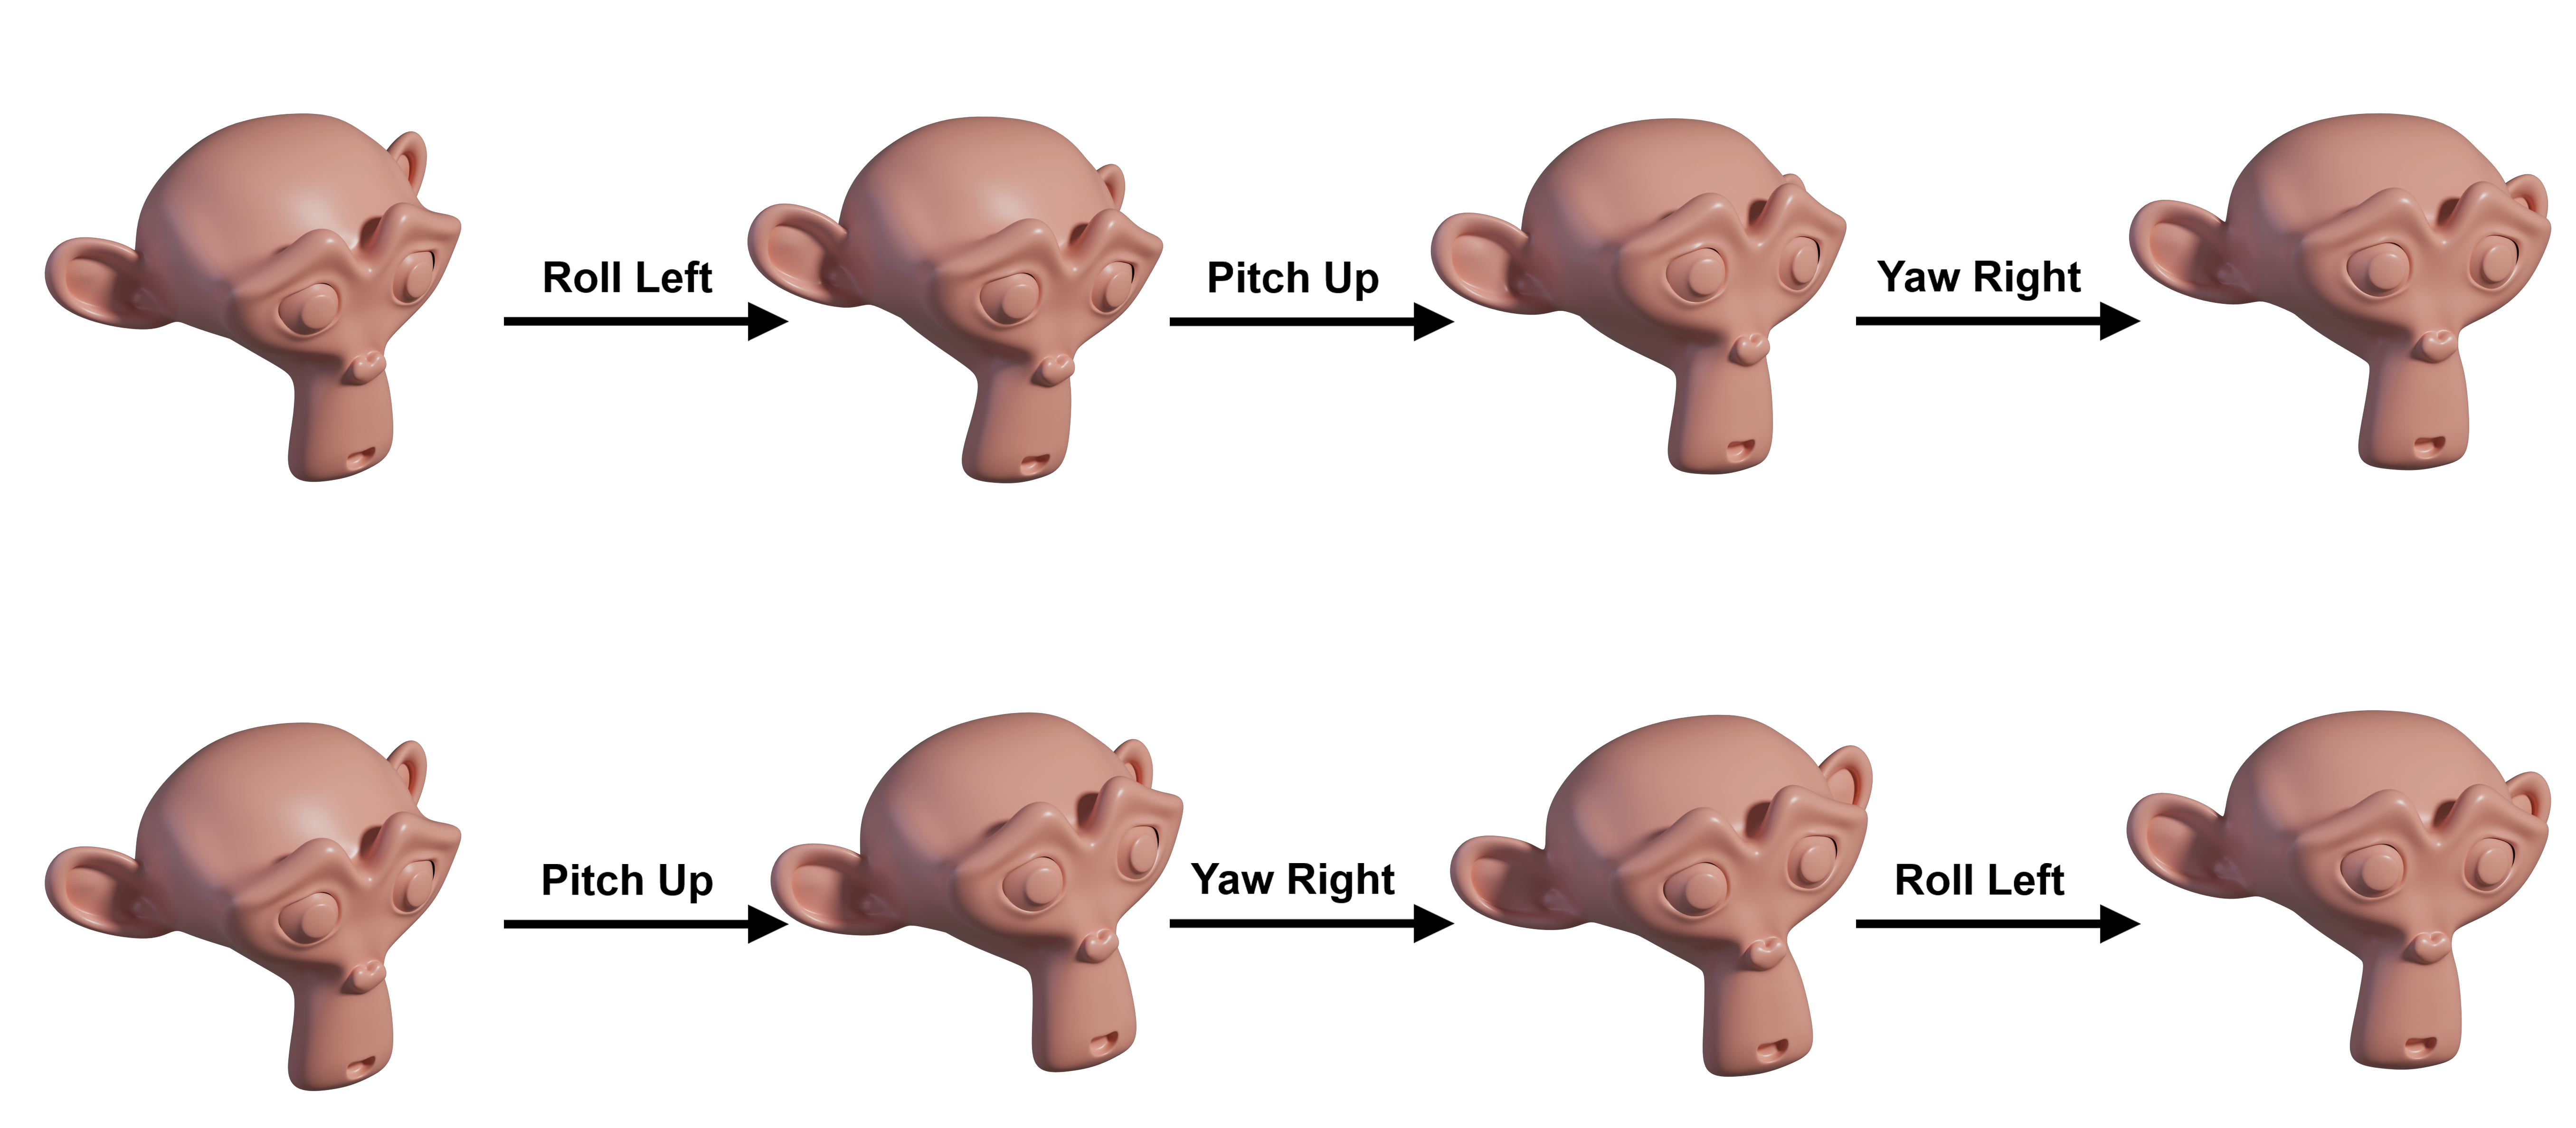
\includegraphics[width=\linewidth]{Images/SmallRotationsExample.png}
    \caption{Example of small rotations being nearly commutative}
    \label{fig:small rot}
\end{figure}
We see that these small rotations yield the same final orientation. Go ahead and try the same rotation sequence with your head! If you choose angles that are fairly small, you will see that you do in fact end up looking in the same spot no matter which rotation sequence you choose! Of course, these two rotations are not \textit{exactly} identical, but they are really close! You can notice some small difference by looking at where Suzanne's' ear intersects with the eyebrow. 

However, these two do seem very similar, which is definitely a different outcome than the large rotations. As we will later prove rigorously, as these rotations get smaller and smaller, these so-called \textit{infinitesimal} rotations will be mathematically identical.

Based on what we've learned from \gls{lie theory} so far, this should give us a few hints as to whats happening. The small rotations are very close to the \gls{lie algebra}, where the elements form a vector space. However, the large rotations exhibit behavior that can only be explained on the manifold. Notice the parallel here with our two dimensional rotations. Even though those two dimensional rotations are commutative and the three dimensional rotations are not, the same principle of infinitesimal rotations holds. The following sections will explain these attributes more mathematically and give special characteristics of rotation groups and algebras.
\end{example}

\subsection{Rotation Groups}
To describe a rotation mathematically, we first need to understand what rotations do. Aside from the obvious fact that rotations `rotate', some properties are inherit no matter what space we rotate in (although 2D and 3D are the most common for us). These properties will help us define the group structure of rotations:

\begin{enumerate}
    \item  Rotations superpose. If we rotate once, and then rotate again, the result is still a rotation, and more importantly, the result is the sum of the first and second rotation.
    \item Secondly, a rotation preserves angles and lengths. By rotating, the length of a vector is never changed. Additionally, the angle between two vectors must also be constant.
    \item Lastly, and likely the most overlooked, rotations preserve the orientations of objects. A pure rotation will never change the order of vectors. This is distinct from a reflection, in which the first two properties hold but the orientation is not preserved.


\end{enumerate}

%Figure for all of these

Each of these have direct mathematical implications. We can go through each of the previously listed properties in order, describing them mathematically:
\begin{enumerate}
    \item The fact that rotations superimpose tells us that a linear representation of then exists -- we can express them in terms of vectors and matrices. Using the other properties, we can ascertain more about the matrix that represents this rotation.
    \item Preserving angles and rotations means that the dot product is constant under a rotation. Assuming that our rotation is denoted $R$, this means that two vectors, $\vec{v}$ and $\vec{w}$ have the following relationship under a rotation:
    \begin{equation}\label{eq:dotty dot prod}
        \vec{v}\cdot \vec{w}=(R\vec{v})\cdot(R\vec{w})
    \end{equation}
    It is known that for real dot products, we can replace the dot product of $\vec{v}\cdot \vec{w}$ with $\vec{v}^\top \vec{w}$ (you can easily prove this to yourself). So, we can rewrite \eqautoref{eq:dotty dot prod} as:
 \begin{equation}
        \vec{v}^\top \vec{w}=(R\vec{v})^\top(R\vec{w})
    \end{equation}
Which can be simplified using the identity that $(R\vec{v})^\top =\vec{v}^\top R^\top $ to:
 \begin{equation}
        \vec{v}^\top \vec{w}=\vec{v}^\top R^\top R\vec{w}
    \end{equation}
For this statement to be true, $R^\top R$ must be equal to the identity matrix, $\mathbb{I}$. The only way this can occur is if:
\begin{enumerate}
    \item R is invertible.
    \item     The transpose of $R$ is it's inverse.
\end{enumerate}
The first statement implies that $R$ must be square (Invertible Matrix Theorem). The second condition that $R^{-1}=R^\top $ is a special condition which implies that the matrix is \textit{orthogonal}. This is a modification of the condition that we saw in \autoref{sec:matrix groups}. In that section, we defined the general linear group $GL(n)$. With the additional constraint that $R^\top =R^{-1}$, we say that rotations exist in the $O(n)$ group. Thus, $O(n) \subset GL(n)$.

    \item The last property is that the orientation and dot products are preserved. Once again, this is the same property that we saw with the special linear group $SL(n)$, and we use the same notation here for the special orthogonal group - denoting it $SO(n)$. As before, the important property with this group is that $\det SO(n) = 1$

\subsection{Rotation Algebras}
    
\end{enumerate}
As mentioned in the introduction to \gls{lie theory}, the \gls{lie algebra} represents the tangent space of the \gls{lie group}. We can intuitively think of the tangent space as taking a derivative. So, we can create our mathematical description of the \gls{lie algebra} for rotations in this way.

We start by taking a differential rotation, one that is very small, which we denote $\varepsilon$. We then use the defining relationship of $O(n)$:
\begin{equation}\label{eq:rotationDef}
    R^\top R=\mathbb{I}
\end{equation}

We can think of $R$ for an infinitesimal rotation. For a very small rotation, the matrix will be only very slightly different from the identity, shifted by some amount $\varepsilon A$, say. Of course, there are some higher order corrections, but choosing $\varepsilon$ to be small, these are insignificant.\endnote{More strictly, we choose $\varepsilon>0$ but so small that $\varepsilon^2=0$. If our rotation is infinitesimal, this is exactly true.} Thus, we can write\endnote{Notice the similarity in this construction and the one for two dimensional rotations we found earlier. We can, in fact, say that this $\varepsilon A$ is the same as the generator matrix which we found for two dimensional rotations.}:
$$R=\mathbb{I}+\varepsilon A$$
The matrix $A$ is representative of the \gls{lie algebra}, the form of which we have yet to define. We can use this relationship in \eqautoref{eq:rotationDef} to find properties of A:
$$(\mathbb{I}+\varepsilon A)^\top (\mathbb{I}+\varepsilon A)=\mathbb{I}$$
We expand the product and ignore any terms with coefficients of $\varepsilon^2$  since these higher order corrections are zero for an infinitesimal transformation. This leads us to:
$$\mathbb{I}+\varepsilon(A^\top +A)=\mathbb{I}$$
From here, the $\mathbb{I}$ matrices cancel, and we are left with the relationship that:
\begin{gather}
    \color{blue}\boxed{\color{black}A^\top =-A}\\
    \color{blue}\mathrm{Skew \ Symmetry}
\end{gather}
This relationship is called \textit{skew symmetry}, and it is the fundamental property of infinitesimal rotations (or the \glspl{lie algebra} of rotations, put another way). One notable feature of skew symmetric matrices is that the diagonal must be zero for the property to hold\endnote{We may identically say that $\det{A}=0$. Remember that for the \gls{lie group}, our determinant was 1, which we may arrive at through $e^0=1$}. We call the \gls{lie algebra} for which this condition holds $\mathfrak{so}(n)$.

We can use the condition on the determinant of the \gls{lie group} to get more information about the \gls{lie algebra}. We know that the determinant of $SO(n)$ must be 1. Therefore, we may have a condition for the $\mathfrak{so}(n)$ \gls{lie algebra} that arises from this. We can use the previously established fact that the trace is related to the matrix exponential determinant (see \autoref{exer:trace det} for more information):
$$e^{tr(A)}=\det\left(e^A\right)$$
The matrix $A$ is the \gls{lie algebra}, and thus $e^A$ is the exponential map, such that $e^A$ is the \gls{lie group}. We have previously determined that the $SO(3)$ \gls{lie group} must have determinant 1, so the equation is:
$$e^{tr(A)}=1$$
Solving the equation by taking the logarithm of both sides, we have:
$$tr(A)=0$$
This condition implies that all of the elements of the diagonal must add to zero! A matrix with such a property is called traceless. Using the other criteria that $A^\top =-A$, each diagonal entry of this matrix must be 0.

The \gls{lie algebra} of the rotation groups appears quite often in engineering and physics. Anytime an infinitesimal rotation must be described a skew symmetric matrix is often associated with it! One example you may remember is the quaternion integration equation from Volume I:
$$\dot{\textbf{q}}=\frac{1}{2}\begin{bmatrix}
        0&-\omega_x&-\omega_y&-\omega_z\\
        \omega_x&0&\omega_z&-\omega_y\\
        \omega_y&-\omega_z&0&\omega_x\\
        \omega_z&\omega_y&-\omega_x&0
    \end{bmatrix}\vec{q}$$
As we can see, this matrix has the properties of the \gls{lie algebra} of rotations! It is skew-symmetric and has a trace of 0.

\subsubsection{The Cross Product and Euler Vector}

Having described the form of the rotation group and the rotation algebra in the context of \gls{lie theory}, we can move on to describing these elements in the more familiar context.



One of the simplest cases in showcasing the relationship between the \gls{lie group} and the \gls{lie algebra} is the rotation.

Starting with an infinitesimal rotation, which is a group in $\mathfrak{so}(3)$, we have:
$$A=\begin{bmatrix}
    0 &-\omega_z & \omega_y \\
    \omega_y & 0 & -\omega_x \\
    -\omega_y & \omega_x & 0
\end{bmatrix}$$

We can use the \gls{exponential map} to go from the \gls{lie group} to the \gls{lie algebra}. For matrices, we use the matrix exponential as the \gls{exponential map}. Performing the exponentiation, we have that $e^{A}$ is a rotation matrix.

\subsubsection{Visualization of SO(3) Rotations}


\subsection{Revisiting the BKE}
We can use \gls{lie theory} in order to describe the \gls{bke} in another way. 
Explain the \gls{bke} in terms of \gls{lie theory}.

\section{Complex Rotations and Spinors}
Until now, we have not discussed complex-valued matrices. However, these find use in physics quite often and we can even parameterize the quaternions in terms of complex matrices. We will now explore these complex matrices to gain an understanding of more complex matrix transformations, which are beyond the 3-D rotations we have discussed so far. These ideas will help us relate the quaternions to rotations and understand how $SU(2)$ and $SO(3)$ space are linked!

This section summarizes some of the ideas that are presented in the \cite{eigenchris_spinors_nodate} playlist of videos.

We may start by considering the 




\section{Physics Applications of Lie Theory}

\subsection{Quantum Mechanics}
\color{red} All quantum mechanical operators are elements of lie algebras! \color{black}

\subsection{Spinors}



\section{Relation to Differential Equations}\label{sec:lie theory relation to differential equations}
We noted in the beginning of this chapter that \gls{lie theory} was originally developed to solve differential equations. We can return back to this example to help us tie the theory into math that almost every engineer has studied extensively.

The foundation of differential equations is, quite naturally, the derivative. Thus, we can start our discussion by showing how the derivative is related to the \gls{lie algebra}.

\subsubsection{Relation to derivatives}
We will start this discussion with the ordinary total derivative that is taught in introductory calculus classes in the context of \gls{lie theory}. Our goal here is to show that the Jacobi identity may arise somewhat naturally by considering the derivative product rule:
$$[f(x)g(x)]'=f(x)g'(x)+f'(x)g(x)$$

Starting with the Jacobi identity, which we know all \glspl{lie algebra} must satisfy, we have:

which can otherwise be expressed as:
$$[x,[y,z]]=-[y,[z,x]]-[z,[x,y]]$$
We have also shown that the Lie bracket is alternating, so we can remove the negative signs on the RHS simply by changing the order of the bracket:
$$[x,[y,z]]=[y,[x,z]]+[[x,y],z]$$

We can rewrite this expression by considering an operation, $D$, which is defined $D(\xi)=[x,\xi]$. Applying this to the equation below, we have:
$$D([y,z])=[y,D(z)]+[D(y),z]$$
Since we consider the Lie bracket to be a type of multiplication, we can write the above formula as:
$$D(yz)=yD(z)+D(y)z$$
Which matches the result of the product rule exactly!

\subsubsection{Differential Equations}
\begin{example}[Matrix Differential Equations]
    Since we have been studying matrix groups, let us consider the class of first order matrix differential equations. We see these systems frequently in control theory so it is good to study them here.
    $$\dot{x}=Ax$$
    Where $A$ is an $n{\times}n$ matrix with constant coefficients and $x$ and $\dot{x}$ are $n{\times}1$ vectors. We can find the solution of this equation through separation and integration. We start by performing the seperation of variables:
    $$\frac{dx}{x}=Adt$$
    We can this integrate this equation to find the solution.
    $$\int_{x_0}^x{\frac{dx}{x}}=\int_{t_0}^\top {Adt}$$
    So, we have $\ln\left(\frac{x(t)}{x_0}\right)=A(t-t_0)$. We note that $t-t_0$ can be replaced by $\Delta t$. Finally, we exponentiate to arrive at our solution to the differential equation:
    \begin{gather}
        \color{blue}\boxed{\color{black}x(t)=e^{A\Delta t}x_0}\\
        \color{blue}\mathrm{Solution \ of \ } \dot{x}=Ax        
    \end{gather}
We can see the presence of the matrix exponential $e^{At}$, which we have seen before when discussing the \gls{lie theory} of matrices! This is an important connection to make, so let us expand on it for clarity.

    Generally, in control theory, we may denote $e^{At}$ (or $e^{A\Delta t}$, they are practically the same) as the \textit{state transition matrix}, which is sometimes denoted $\Phi$. This state transition matrix will extraordinarily important when we discuss concepts such as Kalman filtering.

    So why does it appear here, and how can we relate that to our discussion of \gls{lie theory}?

    We can think of it in the following way. Our matrix $A$ represents infinitesimal behavior of the system. That's why $\dot{x}$ is described in terms of $A$! It tells us how the parameters vary on an infinitesimal scale. The matrix exponential $e^{At}$, is effectively a map from this infinitesimal solution to a finite time solution; that is, something we can measure.

    In \gls{lie theory} we have the exact parallel behavior. We have some tangent group on the \gls{lie algebra}, which is mapped onto the group element by the exponential map!

    We can see that these two descriptions are very similar! The key difference is that \gls {lie theory} can describe groups which are non-linear, which makes is a more powerful tool than solving a linear differential equation.
\end{example}

\section{Lagrangian and Hamiltonians on Manifolds}

\section{Noether's Theorem}\label{Noether's Theorem}

We touched on this briefly in \autoref{sec:motivation and background lie}, but in many physical problems (and in \gls{lie theory}), we are concerned with physical symmetries. Noether's Theorem states the following:

\begin{theorem}[Noether's Theorem]
In a system that can be modeled purely by a Lagrangian (that is, a conservative system), every continuous symmetry has a corresponding conservation law.
\end{theorem}
The implications of this statement are quite great. Noether's Theorem gives us a pathway to understand where the conservation laws of symmetry actually come from. Of course, we can also reverse the statement and understand the symmetries of our system based on the conserved quantities!

Although we have discussed continuous symmetries quite a bit in our discussion of \gls{lie theory}, concrete examples will aid us greatly.

\subsection{Conservation in Physics}

Before we get started, we should concretely define the terminology of the theorem. What exactly do we mean by a conserved quantity?

A conserved quantity is simply one that does not change over time. When we say that energy is conserved, we mean that the energy of the system will be exactly the same if observed at $t=0\ \mathrm{s}$ or $t=100\ \mathrm{s}$. If we call our quantity of interest $X$, we can express this as:
$$\frac{dX}{dt}=0$$

\subsection{Symmetries in Physics}
As we have discussed earlier, the picture of groups and symmetries changes a bit between each domain of math or physics that we are discussing. In the domain of physics, our picture of symmetries is most definitely different than the picture of triangles or number lines.

When we discuss a symmetry in physics, we mean to say that the physics that act upon that system are in no way altered by whatever transformation we have performed (that is to say, the \gls{eom} is identical).

For example, if we decide to move our rocket launch 20 ft to the north, the aerodynamics, gravity, and forces of the rocket are still exactly the same. We have performed a transformation -- in the form of moving the launch location -- but there are no observable differences to the system!

Of course, these transformations are not merely limited to physical movements of the system, there are other types of transformations that we can do that do not impact the physics of the system.

\subsection{The Mathematical Formulation}

We know from Hamilton's Principle that physical trajectories have an action of zero. We denote this action as $S$, and the path it follows as $\gamma$, so we may write $S[\gamma]=0$. It may be possible to find another path $S[\gamma_2]=0$ somewhere else along the state space. This is not particularly noteworthy. We can take the analogy of the derivative from calculus as an example in \autoref{fig:calc sym}:
\begin{figure}[H]
    \centering

\tikzset{every picture/.style={line width=0.75pt}} %set default line width to 0.75pt        

\begin{tikzpicture}[x=0.75pt,y=0.75pt,yscale=-1,xscale=1]
%uncomment if require: \path (0,300); %set diagram left start at 0, and has height of 300

%Shape: Polynomial [id:dp5733809673289914] 
\draw  [line width=1.5]  (100,225) .. controls (170,35) and (240,320) .. (310,130) ;
%Shape: Polynomial [id:dp22075841317731382] 
\draw  [line width=1.5]  (310,130) .. controls (383.33,-100) and (456.67,245) .. (530,15) ;
%Straight Lines [id:da16902943176946206] 
\draw [color={rgb, 255:red, 74; green, 144; blue, 226 }  ,draw opacity=1 ][line width=1.5]    (210,199) -- (290,199) ;
%Straight Lines [id:da8215493758509421] 
\draw [color={rgb, 255:red, 74; green, 144; blue, 226 }  ,draw opacity=1 ][line width=1.5]    (430,99) -- (510,99) ;
%Straight Lines [id:da24241399926680518] 
\draw [color={rgb, 255:red, 218; green, 44; blue, 0 }  ,draw opacity=1 ]   (320,95) -- (280,65) ;
%Straight Lines [id:da37036162717673604] 
\draw [color={rgb, 255:red, 218; green, 44; blue, 0 }  ,draw opacity=1 ]   (400,240) -- (468.58,112.64) ;
\draw [shift={(470,110)}, rotate = 118.3] [fill={rgb, 255:red, 218; green, 44; blue, 0 }  ,fill opacity=1 ][line width=0.08]  [draw opacity=0] (8.93,-4.29) -- (0,0) -- (8.93,4.29) -- cycle    ;
%Straight Lines [id:da8857104314835499] 
\draw [color={rgb, 255:red, 218; green, 44; blue, 0 }  ,draw opacity=1 ]   (350,250) -- (262.74,211.22) ;
\draw [shift={(260,210)}, rotate = 23.96] [fill={rgb, 255:red, 218; green, 44; blue, 0 }  ,fill opacity=1 ][line width=0.08]  [draw opacity=0] (8.93,-4.29) -- (0,0) -- (8.93,4.29) -- cycle    ;
%Straight Lines [id:da5379556180362811] 
\draw [color={rgb, 255:red, 74; green, 144; blue, 226 }  ,draw opacity=1 ]   (250,199) ;
\draw [shift={(250,199)}, rotate = 0] [color={rgb, 255:red, 74; green, 144; blue, 226 }  ,draw opacity=1 ][fill={rgb, 255:red, 74; green, 144; blue, 226 }  ,fill opacity=1 ][line width=0.75]      (0, 0) circle [x radius= 2.34, y radius= 2.34]   ;
%Straight Lines [id:da1048842221660955] 
\draw [color={rgb, 255:red, 74; green, 144; blue, 226 }  ,draw opacity=1 ]   (470,99) ;
\draw [shift={(470,99)}, rotate = 0] [color={rgb, 255:red, 74; green, 144; blue, 226 }  ,draw opacity=1 ][fill={rgb, 255:red, 74; green, 144; blue, 226 }  ,fill opacity=1 ][line width=0.75]      (0, 0) circle [x radius= 2.34, y radius= 2.34]   ;

% Text Node
\draw (354,242.4) node [anchor=north west][inner sep=0.75pt]  [color={rgb, 255:red, 218; green, 44; blue, 0 }  ,opacity=1 ]  {$f'=0$};
% Text Node
\draw (249,47.4) node [anchor=north west][inner sep=0.75pt]  [color={rgb, 255:red, 218; green, 44; blue, 0 }  ,opacity=1 ]  {$f( x)$};


\end{tikzpicture}

    
    \caption{Calculus Analogy of Discrete Symmetry}
    \label{fig:calc sym}
\end{figure}
Given a general function, it is expected that there will likely be multiple minima, separated spatially. What Noether's Theorem is concerned with is infinitesimal transformations that do not change the action at all. In the case of our example before, we have some transformation, which we may call $T$, which maps path $\gamma$ to $\gamma'$:
$$\gamma\xrightarrow{T}\gamma'$$
When we have a continuous symmetry between these two, there is no difference in the action! So $S[\gamma]=S[\gamma']$.

\section{The Limitations of Lie Theory}
A fundamental understanding of the mathematics that relate groups and algebras is quite interesting, but ultimately, our goal in engineering is to be able to control a system which is not mathematically ideal. We will have disturbances and random behaviors and noisy sensors in all of our real systems. Do these non-idealities make \gls{lie theory} useless for us? Of course not, but it does impose limitations of the extent to which we can use it.

It is best to think of \gls{lie theory} as a tool that we can use to understand the relationships between infinitesimal elements and the larger system behavior that we see. From \gls{lie theory}, we can derive a large number of theoretical conclusions (and some which are still active research!) which prove useful to us. Understanding where our theoretical results come from can help us to understand new systems and generate methods of tackling difficult problems. That alone makes \gls{lie theory} a topic worth serious exploration.

Lie Theory, however, is not a silver bullet which can solve all of our practical problems. Quite notably, the computation of matrix exponentials and general exponential functions can be quite expensive and unintuitive, so it often cannot be used in real time systems. From here, we will use \gls{lie theory} mostly to contextualize some of the background and behind the scenes mathematics. 

\newpage

\printendnotes


\chapter{Symplectic Integrators}\label{sec: Syplectic Ints}
In addition to the standard \gls{numerical int} schemes explored in Volume I, there are a variety of integration schemes that use energy conservation as the basis of their integration schemes. These types of integrators are called \glspl{symplectic int} and \glspl{variational int}. These types of integrators directly solve Hamilton's equations for a \gls{Hamiltonian} system. The form of these equations is discussed in \autoref{chap:hamiltonian}.

Because the \gls{Hamiltonian} equations are first order already, they are ready for numerical integration without the need for order reduction.

A similar operation can be done to reduce the \gls{Lagrangian} to two first order equations, in a system known as a variational integrator.

MATLAB has no built in functions for variational or \glspl{symplectic int}, so to implement them we need to discuss their properties in full. 

\section{The Mathematical Background}
Our discussion will build off the mathematical discussion of the \gls{lie group}, so a thorough reading of \autoref{chap:lie theory} is recommended. We will use properties of the $SL(n)$ group as well as some new features.

We will construct a group called the \textit{Symplectic Linear Group} to do this. We define the group as follows:
\begin{gather}
    Sp(2n)\equiv\left\{\psi\in GL(2n,\mathbb{R})|\psi^\top \Omega\psi=\Omega\right\}\\
    \mathrm{where  \ } \Omega=\begin{bmatrix}
        0&I(n)\\-I(n)&0
    \end{bmatrix}
\end{gather}
We can deconstruct the meaning of the line to be: The symplectic linear group is a group, such that set $\psi$, which is a subset of the general linear group $GL(2n,\mathbb{R})$, satisfies the property that $\psi^\top \Omega\psi=\Omega$.

Moreover, $Sp(2n)$ is a \gls{lie group}!


\section{Implementation}


\subsubsection{Use Case of Symplectic Integrators}
Although MATLAB does not have built-in functions for these integrators, scripts to do so can be written or found online.

The best use case for these algorithms is for systems with a \gls{Hamiltonian} or \gls{Lagrangian} description that need to be integrated over a long time span. Because these integrators conserve energy, they will better preserve the characteristics of these systems over long times as compared to RK integrators.

\chapter{The Lebesgue Integral and Measure}

\begin{chapquote}{Andrew Lewis}
``The Lebesgue theory of integration is to the Riemann theory of integration as the real numbers are to the rational number''
\end{chapquote}

In the interest of keeping \autoref{part:control theory} free of too much strictly mathematical content, I have devised this chapter which contains much of the math which is foundational in classical control theory.

For the reader interested in the mathematics behind inner product spaces, I have included some supplemental information on the Lebesgue integral, which is the mathematical construction that is used to rigorously define inner product spaces.




\section{Field Theories}

To describe field theories, we should first return to the \gls{Lagrangian} which we have discussed earlier. So far, we have discussed discrete systems. That is, systems which we can describe with a finite number of degrees of freedom.

What happens if we instead try to model something which is continuous? In our applications, we can approximate any fluid as continuous. In physics, gravitational fields and electromagnetic fields are continuous. 

\chapter{A Brief Tour of Complex Analysis}
\begin{chapquote}{Jacques Hadamard}
    The shortest path between two truths in the real domain passes through the complex domain.
\end{chapquote}


\chapter{Tensor Operations}
Before we dive into differential geometry or any of the related topics, we must first have a good understanding of tensors and their operations.

\chapter{Differential Geometry}
Differential geometry is a field of study that is concerned with the study of smooth manifolds - which essentially means that it is an object which `looks' like a vector space when viewed closely. The subject of differential geometry was lightly touched upon in \autoref{ex:geodesic}, where we considered the shortest path on a spherical surface. In \autoref{ex:geodesic}, we showed this property on the sphere, but differential geometry allows us to study any manifold, so long as it is smooth! 

As we have seen, smooth manifolds are quite important to \gls{lie theory}, and many other applications as well. It is thus sagacious to devote a chapter to a study of differential geometry. We find that many physical systems can be described by the methods of differential geometry.

We can think of a manifold as anything which we can continuously parameterize. So, our 3D rotations that we parameterize with Euler angles or quaternions are also elements of a manifold. We also see that manifolds are also useful in \gls{Lagrangian} and \gls{Hamiltonian} mechanics in the form of \textit{symplectic manifolds}.

So, this is a field of study that touches upon many of the mathematical concepts that we encounter in the study of dynamics and control theory. While not strictly necessarily, a preliminary understanding of manifolds will prove useful for further study. Moreover, those readers interested in physics will find many uses for the topics of discussion here.

This chapter will take an approach closer to physics rather than pure math, as the math requires knowledge of topology and analysis which are well outside the scope of this book and the expected knowledge of the target audience. However, useful information and a working knowledge of the subject can be gained nonetheless from a slightly less -- but still informative -- approach to the subject.

\section{Invariance, Covariance \& Contravariance }

Change of basis and change of component matrices are inverses of each other. Seen with scaling, rotations, etc.

Quantities that act in the opposite direction as the basis vectors are contravariant, those that act the same are covariant. There \textbf{must} be an inverse relationship between covariant and contravariant quantities to maintain the same value. 

Quantities which are unchanged are invariant. Tensors are invariant quantities! Can be described differently, but the properties never change

covariant - row
contravariant - column


\subsection{The Metric Tensor}
The concept of a metric is of upmost importance to differential geometry. A metric space is a set with a notion of a distance.

The most typical metric space is the Euclidean $\mathbb{R}^2$ space. The distance in this space is perhaps the most famous distance formula to exist:
$$s=\sqrt{x^2+y^2}$$

\subsection{Distances}
We can generalize the concept of the Euclidean distance, which we typically define as
$$s=\sqrt{x^2+y^2}$$
In a generic metric space, we can define this as
$$s=\int_a^b\sqrt{g_{ij}\frac{dx^i}{d\lambda}\frac{dx^j}{d\lambda}}d\lambda$$
\subsubsection{Applying Euler-Lagrange}
We notice that the form of the equation for the arc-length matches the form of a functional in \gls{Lagrangian} mechanics! We can apply the Euler-Lagrange equation to get a general equation for the geodesic on any surface!

$$\frac{d^2x^i}{d\lambda^2}+\Gamma_{mn}^i\frac{dx^m}{d\lambda}\frac{dx^n}{d\lambda}=0$$

\section{The Lie Derivative}




\section{Special Relativity}

\section{General Relativity}

\chapter{Geometric Control}


